\documentclass[11pt,a4paper]{article}
\usepackage[margin=3cm]{geometry}
\usepackage[utf8]{inputenc}
\usepackage{courier}
\usepackage{amsmath}
\usepackage{amsfonts}
\usepackage{amssymb}
\usepackage{makeidx}
\usepackage{graphicx}
\usepackage{hyperref}
\usepackage{indentfirst}
\usepackage{xcolor}
\usepackage{epsfig}
\usepackage{listings}
% -- subtitle
\usepackage{titling}
\newcommand{\subtitle}[1]{%
	\posttitle{%
		\par\end{center}
	\begin{center}\large#1\end{center}
	\vskip0.5em}%
    % http://tex.stackexchange.com/questions/50182/subtitle-with-the-maketitle-page
}
% -- fonts
\usepackage{fontspec}
\setmainfont{RomanSerif}
\setsansfont{Overlock}
\setmonofont{Inconsolata}
% -- xmark
\newcommand{\xmark}{\textcolor{green!50!black}{x}}
% -- table font size -- http://tex.stackexchange.com/questions/27097/changing-the-font-size-in-a-table
\usepackage{floatrow}
\DeclareFloatFont{large}{\large} % "scriptsize" is defined by floatrow, "tiny" not
\floatsetup[table]{font=large}
% -- author, title
\author{}
\title{24+Radio Catalog Manual}
\subtitle{(GOODS-North)}
\begin{document}
\maketitle
\tableofcontents
\clearpage
\setlength{\baselineskip}{16pt}
\setlength{\parskip}{5pt}
% -- code style text box
\lstset{
	numbers=left,
	stepnumber=1,
	numbersep=10pt,
	numberstyle=\footnotesize,
	basicstyle=\fontsize{8}{12}\ttfamily,
	keywordstyle=\color{blue!70},
	commentstyle=\color{red!50!green!50!blue!50},
	frame=shadowbox,
	rulesepcolor=\color{red!20!green!20!blue!20},
	escapeinside=``,
	xleftmargin=2em,
	xrightmargin=0em,
	aboveskip=1em,
	tabsize=4,
	showspaces=false,
	showstringspaces=false
}

%*************************************************************************************
\section{Abstract}

This is the manual for the 24+radio catalog. We select sources from the GOODS-Spitzer IRAC catalog in GOODS-North field using 24 and radio images. 

We use Monte-Carlo simulation to validate and correct measurements. The output is a catalog contains IRAC, Ks, 24 and radio band flux and uncertainties. Additional, we measure 16um based on this catalog, and append 16um flux and uncertainty to our final 24+radio catalog. 

With the final 24+radio catalog, we do a panchromatic SED fitting to derive SFR, dust mass, and to predict the far-infrared band fluxes, which will be used for the next step ''super-deblending'' photometry. 

\vspace{5cm}
Hints: black text are our method and procedures, \textcolor{blue}{blue text are notes}, and \textcolor{red}{red text are unsolved issues.}

%*************************************************************************************

\clearpage

%*************************************************************************************
\section{Band 24}

\subsection{Galfit at band 24}

We use these commands to run the galfit photometry at band 24:

\begin{lstlisting}[language=bash]
# run first-pass without varying source position
./do_Galfit 24 201500 -catalog irac_mips_fluxes_hdfn.dat
ssh planer; cd boxgalfit; do_GalfitRunqsub; cd ..; exit
./do_Galfit 24 201500 -catalog irac_mips_fluxes_hdfn.dat -postparallel
# then second-pass varying source position
./do_Galfit 24 201500 -catalog irac_mips_fluxes_hdfn.dat -vary
ssh planer; cd boxgalfit_vary; do_GalfitRunqsub; cd ..; exit
./do_Galfit 24 201500 -catalog irac_mips_fluxes_hdfn.dat -vary -postparallel
\end{lstlisting}

Before running this please make sure that the computer meets the software dependencies in Section \ref{Appendix_Software_Dependencies}. 

The input is the catalog, the sci fits image, rms fits image and psf fits image. The latter 3 images are set in "goFine.sm": 

\begin{lstlisting}[language=bash]
# goFine.sm
xSet_24	define imax 24
		define imax_name "n_mips_1_s1_v0.37_sci_BS"  # subtracted median smooth back
		define imax_name_rms "n_mips_1_s1_v0_37_rms_ED"
		define imax_name_psf "hdfn_dao_mipspsf"
		define xdate "201500" # the data processing date or version
\end{lstlisting}

The input of the bash script "do\_Galfit" are: 

\begin{lstlisting}[language=bash]
# do_Galfit
./do_Galfit \
	24 \ 		# this overwrites "define imax 24" in goFine.sm xSet_24
	201500 \ 	# this overwrites "define xdate 201500" in goFine.sm xSet_24
	-catalog XXXX \ # the catalog, with columns id, ra, dec
	-fitsname XXXX \ # this overwrites "define imax_name XXXX" in goFine.sm xSet_24
	-vary \ 	# this overwrites "define vary_positions 1" in goFine.sm xSet_24
\end{lstlisting}

The process of the bash script "do\_Galfit" is basically reproducing the "xFit\_24" function in "goFine.sm":

\begin{lstlisting}[language=bash]
# goFine.sm
xFit_24	xSet_24
		data catalog
		read idF raF deF
		Fit_XXX
		Rebuild_XXX
		# -- it takes quite a long time to finish the galfit processes
		#    becuase we divide the large image into small boxes 
		#    and run galfit in each box one by one
		# -- alternatively, we can run the galfit parallelly 
		#    for all boxes with the help of supercomputer "planer", 
		#    that is, we first generate the files of all boxes, 
		#    then launch galfit parallelly on "planer" for all boxes, 
		#    finally combine all boxes and call "Rebuild_XXX"
		#    to generate the output data products. 
		# define doParallel 1 # this is new added function for running parallely
		# Fit_XXX
		# define doPostParallel 1 # this is new added function for running parallely
		# Fit_XXX
		# Rebuild_XXX
\end{lstlisting}

The output of the bash script "do\_Galfit" are: 

\begin{lstlisting}[language=bash]
FIT_goodsn_24_Map_201500.fits	# This output fits file contains 3 images: 
								# the original input image, 
								# the best fitted source model image, 
								# and the residual image. 
								# One can notice that there are some faint tile 
								# features, which are because we are mosaicing all 
								# the small boxes together to get the final data 
								# product. (A remodelling of all sources over the 
								# full map will certainly remove these features.)
FIT_goodsn_24_Map_201500_vary.fits	# This output fits file is similar to the above 
									# one, just it is fitted by allowing bright 
									# sources to slightly vary their positions. 
results_24_201500			# The output ascii table containing x, y, noise (rms), 
							# magnitude, error, id, ra, dec, etc. 
results_24_201500.info		# The output text file containing goFine.sm parameter. 
results_24_201500_vary		# The output ascii table containing same columns as above, 
							# for the fitting allowing bright sources to vary positions. 
results_24_201500_vary.info	# The output text file containing goFine.sm parameters, 
							# for the fitting allowing bright sources to vary positions. 
\end{lstlisting}

Clearly, the output of galfit is magnitude and error in magnitude, 
therefore we need to convert magnitude into flux. 
This can be done in either "goFine.sm R\_MIPS24" function, 
or "astroPhot.sm convert\_mag2flux" function. 

Moreover, galfit output errors (uncertainties) are found not 
fully representing the actual errors e.g. in simulations, 
therefore we need to correct or compensate galfit errors, 
with the help of Monte-Carlo simulations (in next Section) and the simulation analyses (the Section after next Section). 




\subsection{Galsim at band 24}

We use these commands to run the Monte-Carlo simulation at band 24:

\begin{lstlisting}[language=bash]
sm
load astroPhot.sm # `{\color{gray}\fontsize{5}{5}{\url{https://github.com/1054/DeepFields.SuperDeblending/blob/master/Softwares/Supermongo_macro/astroPhot.sm}}}`
# first estimate magnitude range
convert_flux2mag goodsn 24 $(0.0044*01) 1 # (mBias -0.2036 fBias -0.000553)
convert_flux2mag goodsn 24 $(0.0044*25) 1 # (mBias -0.2036 fBias -0.000553)
# then do the simulation
./do_Galsim 24 201500 -mag0 -2.8416 -mag1 0.530157 -number 6000 -vary \
-catalog irac_mips_fluxes_hdfn.dat
ssh planer; cd boxgalsim; do_GalsimRunqsub; cd ..; exit
./do_Galsim 24 201500 -mag0 -2.8416 -mag1 0.530157 -number 6000 -vary \
-catalog irac_mips_fluxes_hdfn.dat -postparallel
\end{lstlisting}

\subsection{Galsim Analysis at band 24}

We use these commands to run the simulation analysis at band 24:

\begin{lstlisting}[language=bash]
sm
macro read run_simu_stats_v7.sm run_simu_stats_v7 24 201500
\end{lstlisting}

Below are our statistical analyses:

\begin{figure}[H]
	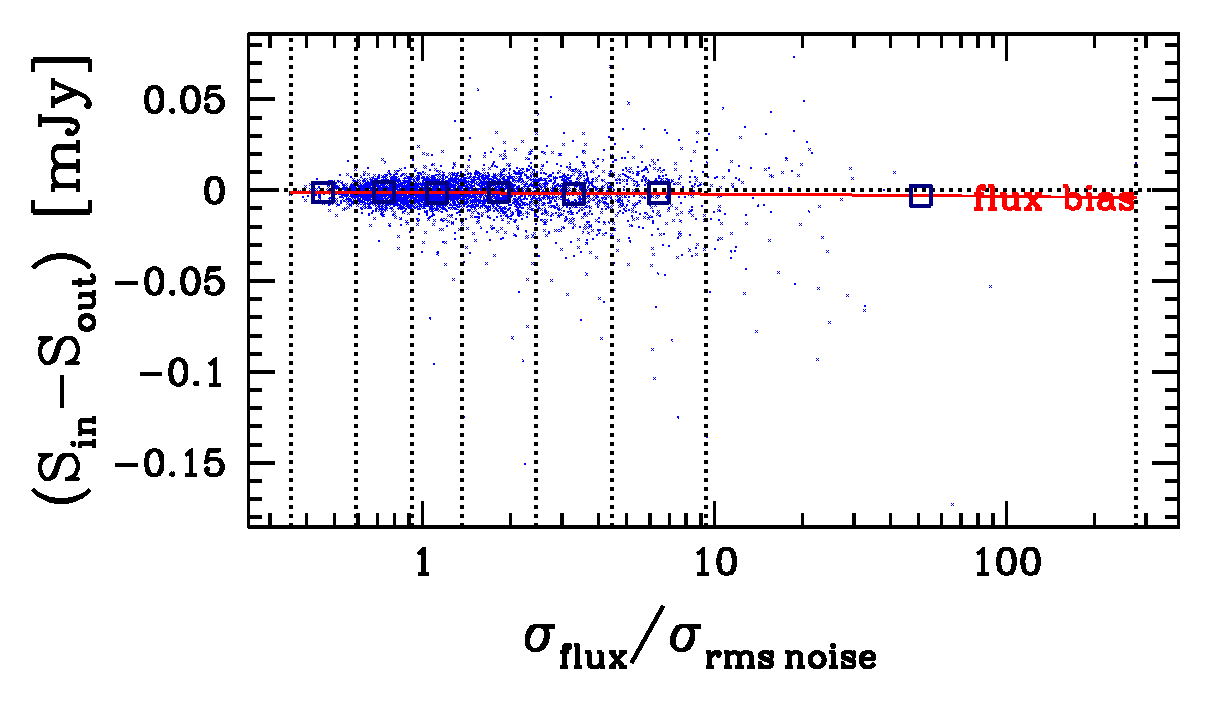
\includegraphics[width=0.8\textwidth]{galsim_24_fbias_1}
	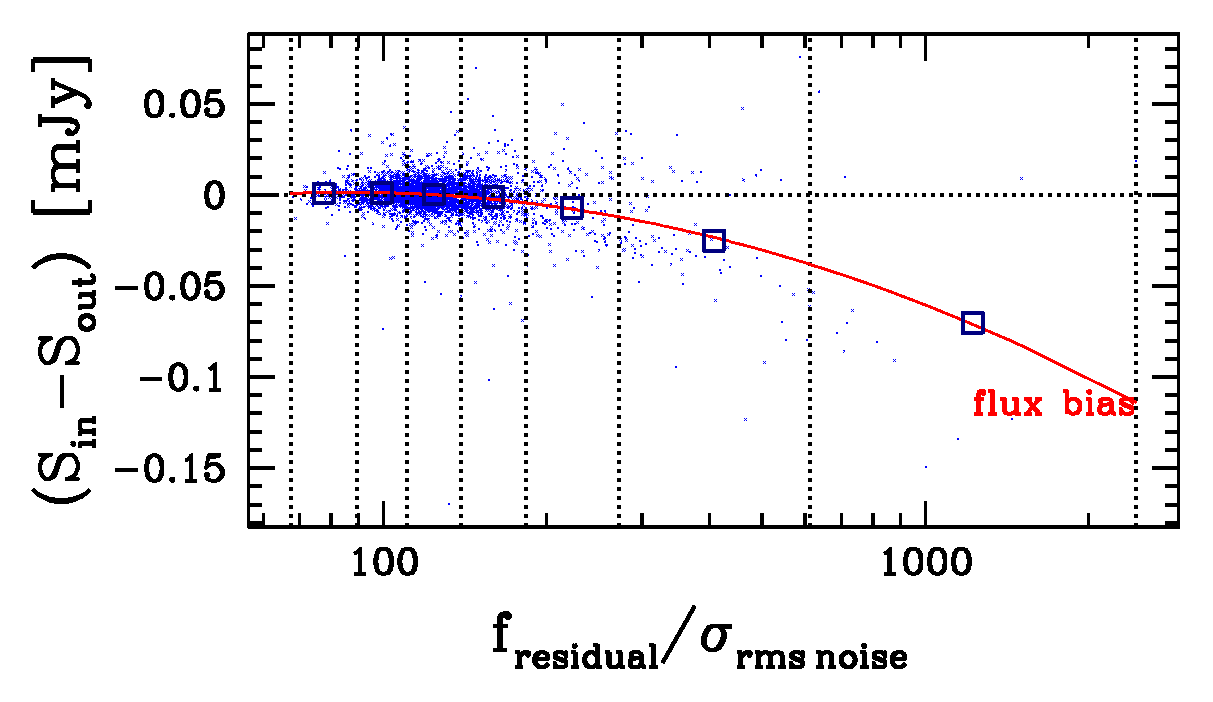
\includegraphics[width=0.8\textwidth]{galsim_24_fbias_2}
	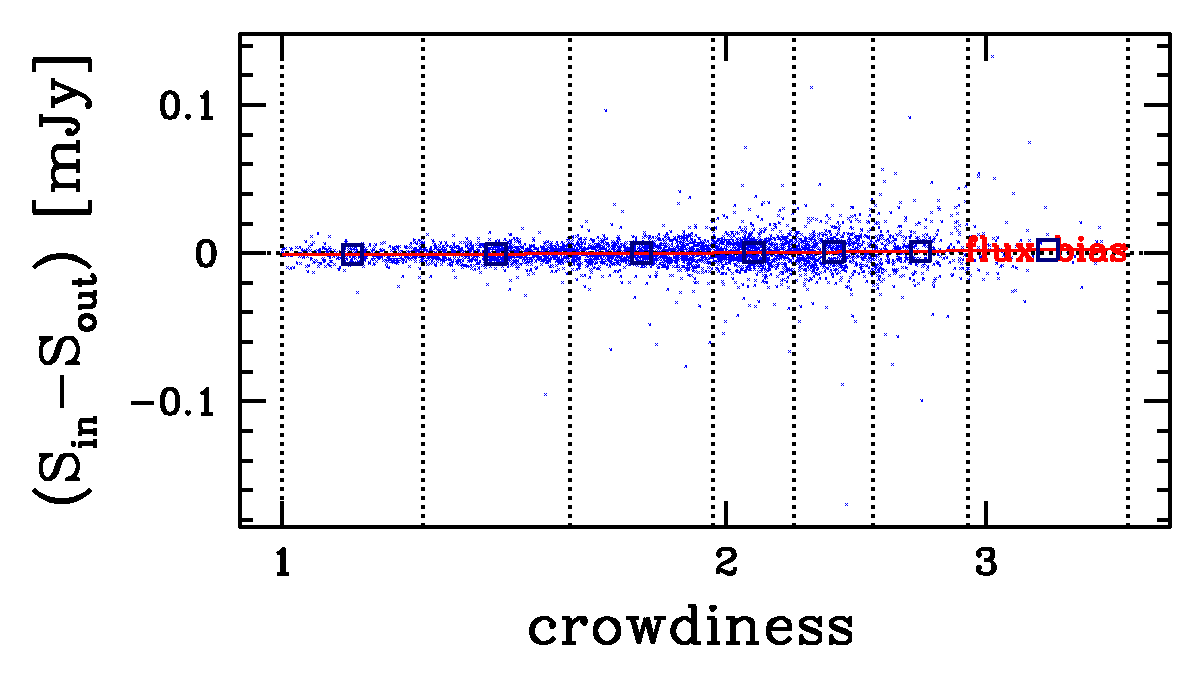
\includegraphics[width=0.8\textwidth]{galsim_24_fbias_3}
	\caption{Flux bias analysis from simulation.}
\end{figure}

\begin{figure}[H]
	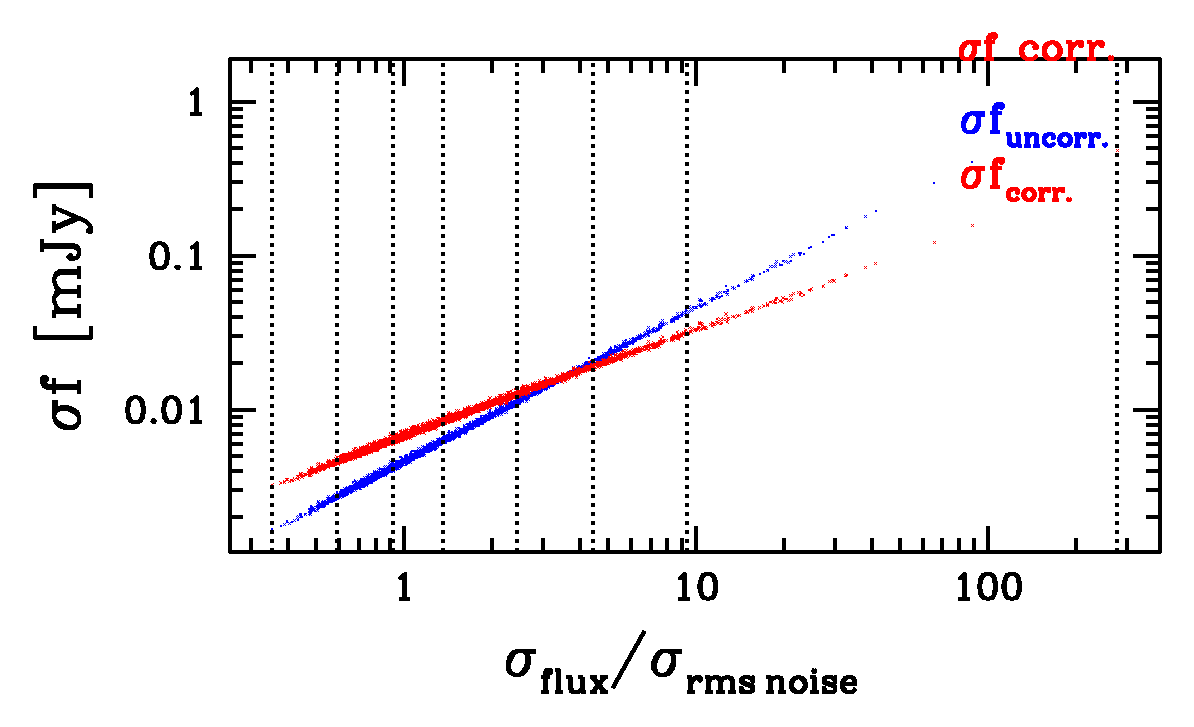
\includegraphics[width=0.8\textwidth]{galsim_24_dfcorr_1}
	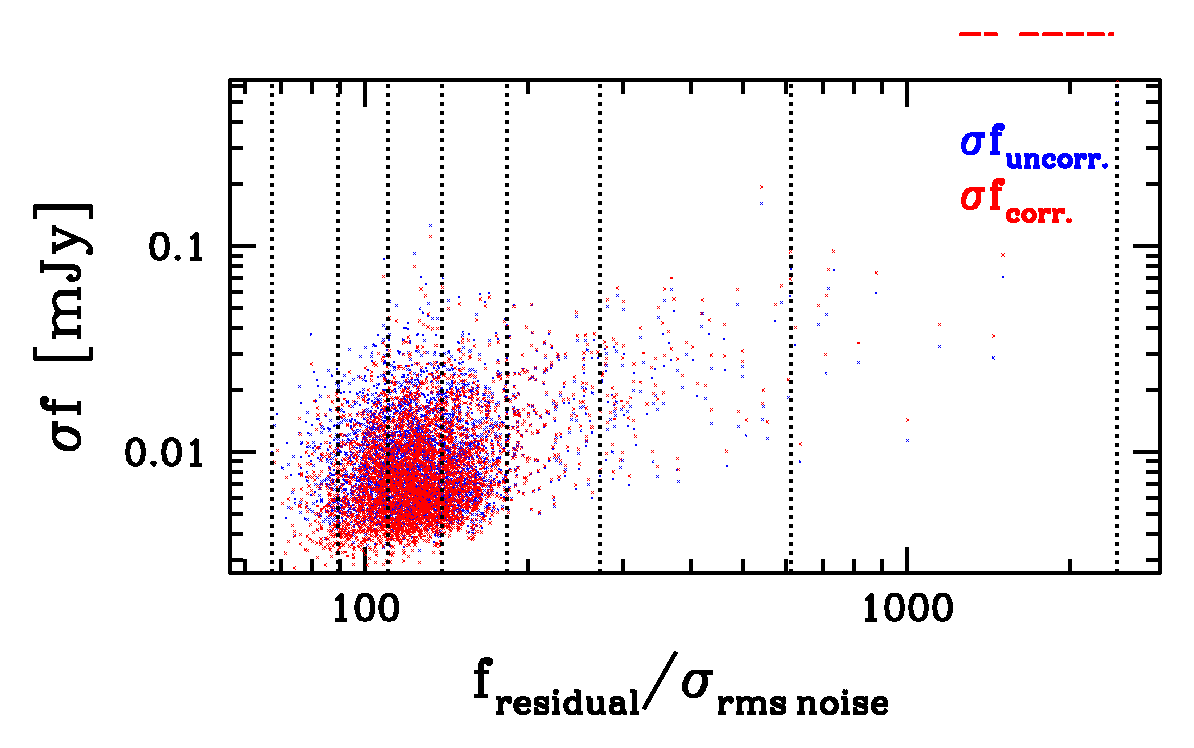
\includegraphics[width=0.8\textwidth]{galsim_24_dfcorr_2}
	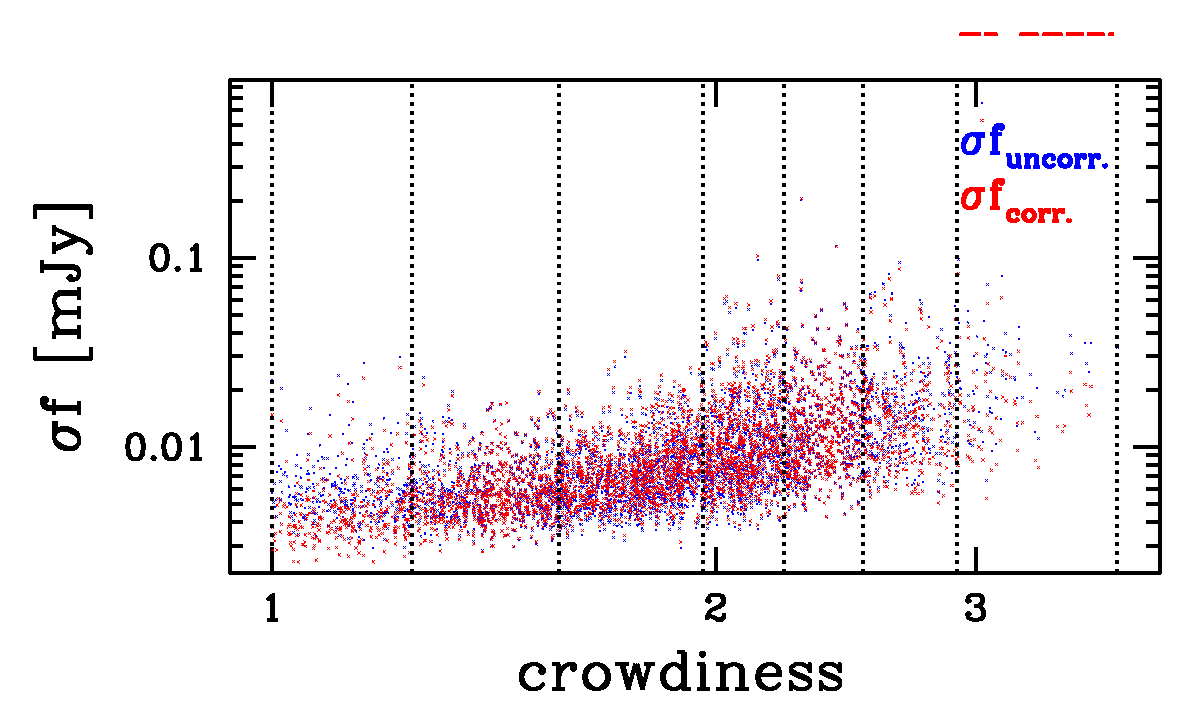
\includegraphics[width=0.8\textwidth]{galsim_24_dfcorr_3}
	\caption{Flux uncertainty analysis from simulation.}
\end{figure}

\begin{figure}[H]
	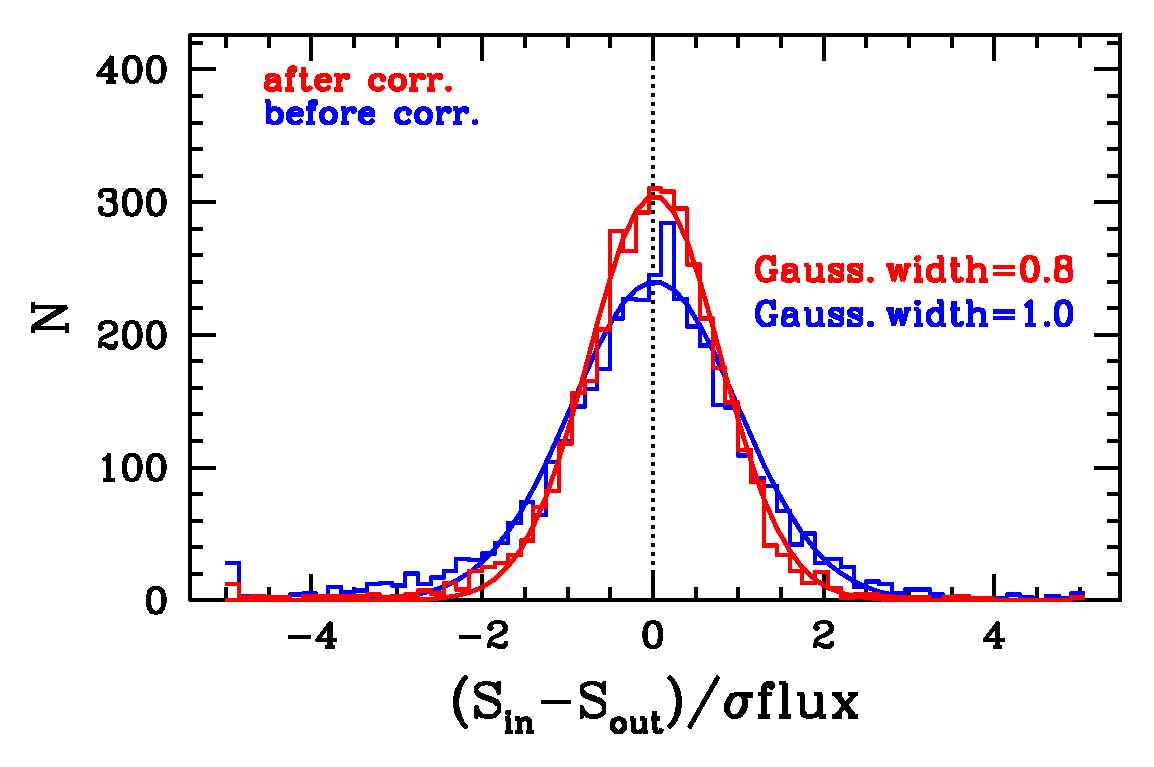
\includegraphics[width=0.75\textwidth]{galsim_24_hist_dfcorr_1}
	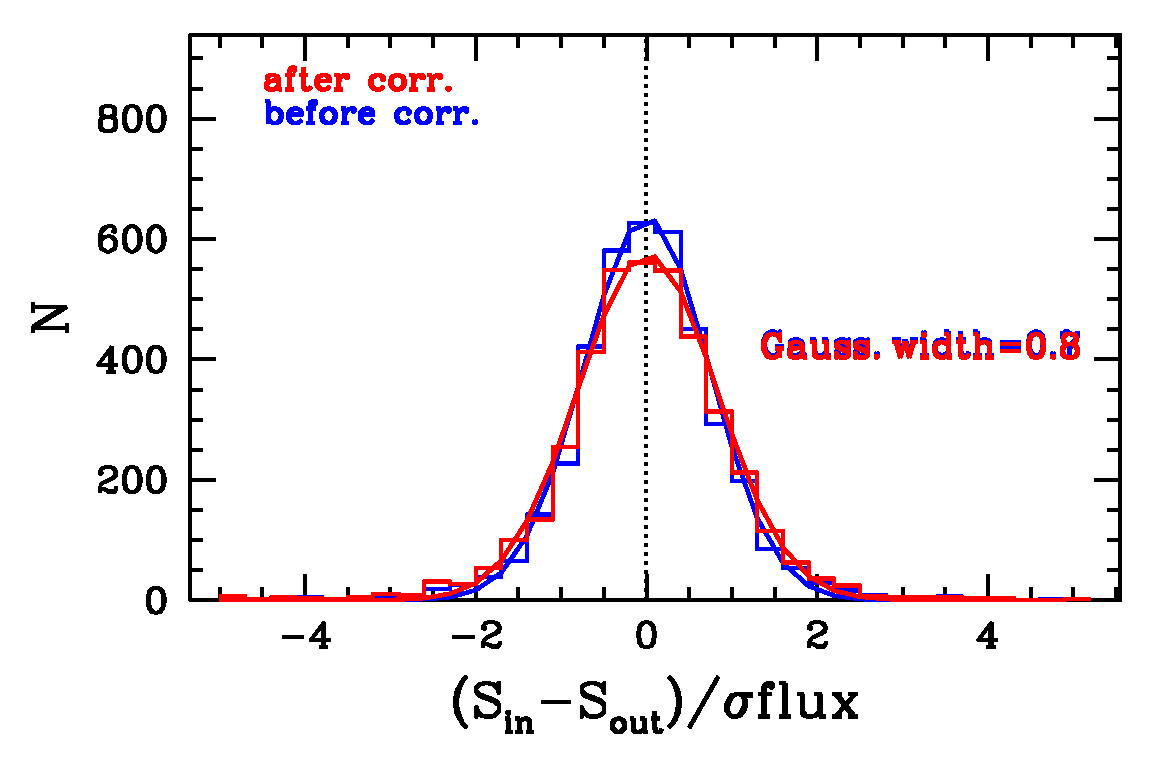
\includegraphics[width=0.75\textwidth]{galsim_24_hist_dfcorr_2}
	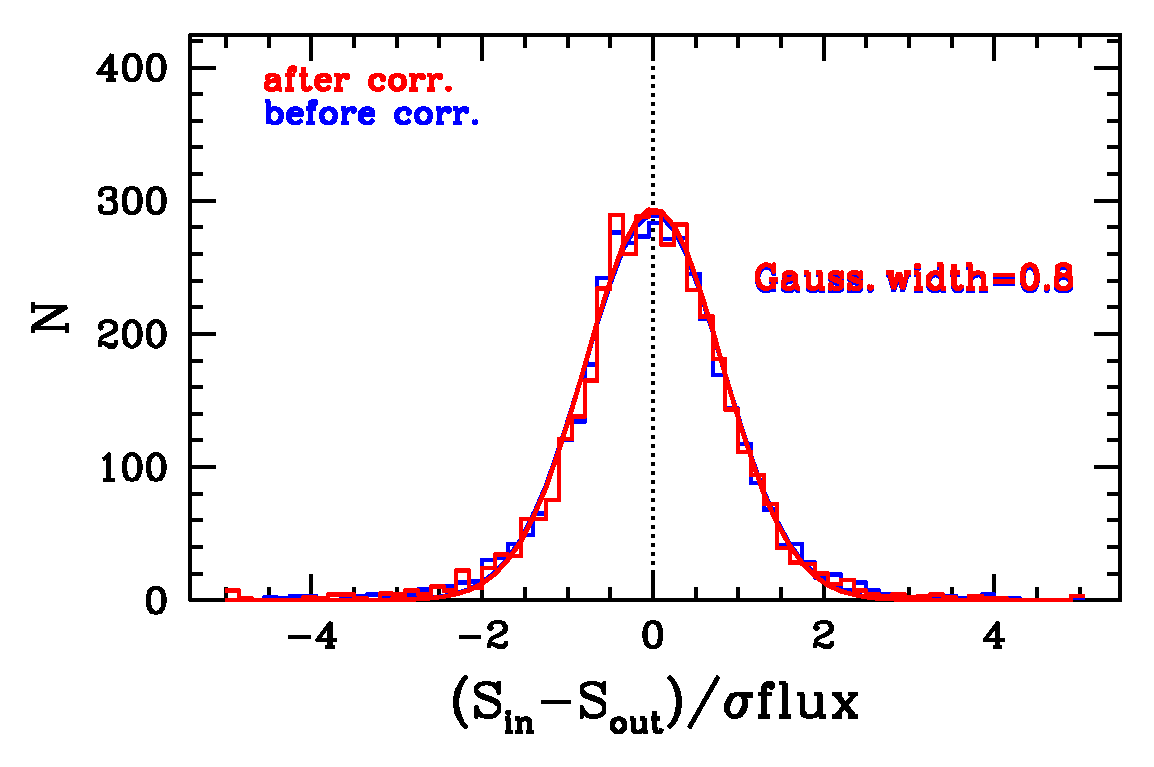
\includegraphics[width=0.75\textwidth]{galsim_24_hist_dfcorr_3}
	\caption{Statistical behavior of input minus output differences before and after correction.}
\end{figure}




\subsection{Comparing the measurements with literature at band 24}

\begin{figure}[H]
	\includegraphics[width=0.75\textwidth]{compare_f24_dzliu_with_daddi_20160119}
	\includegraphics[width=0.75\textwidth]{compare_f24_dzliu_with_daddi_log_20160119}
	\caption{Comparing the new dzliu 2015 measurements with daddi 2014 measurements ($f_{24}$). Note that dzliu 2015 have applied new simulation-based flux bias and flux error correction recipes, but all sources were only fitted with PSF functions rather than Gaussian or S\'{e}rsic, therefore the few brightest sources have lower fluxes. \textcolor{red}{TODO: improve the fitting with Gaussian functions. But should we simulate Gaussian shape sources in simulations? Will the simulation correction recipes be biased for Gaussian shape sources?}}
\end{figure}

\begin{figure}[H]
	\includegraphics[width=0.75\textwidth]{compare_f24_dzliu_with_elbaz_2013_20160119}
	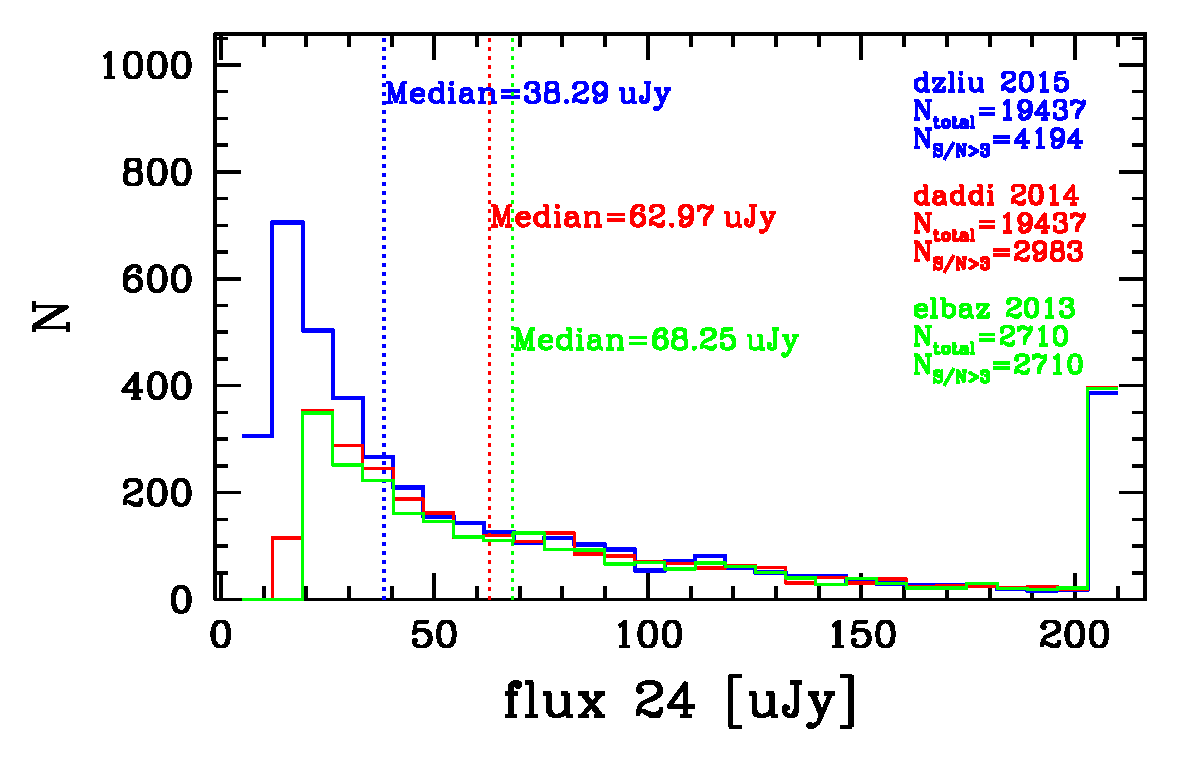
\includegraphics[width=0.75\textwidth]{compare_f24_histogram_dzliu_daddi_elbaz_20160124}
	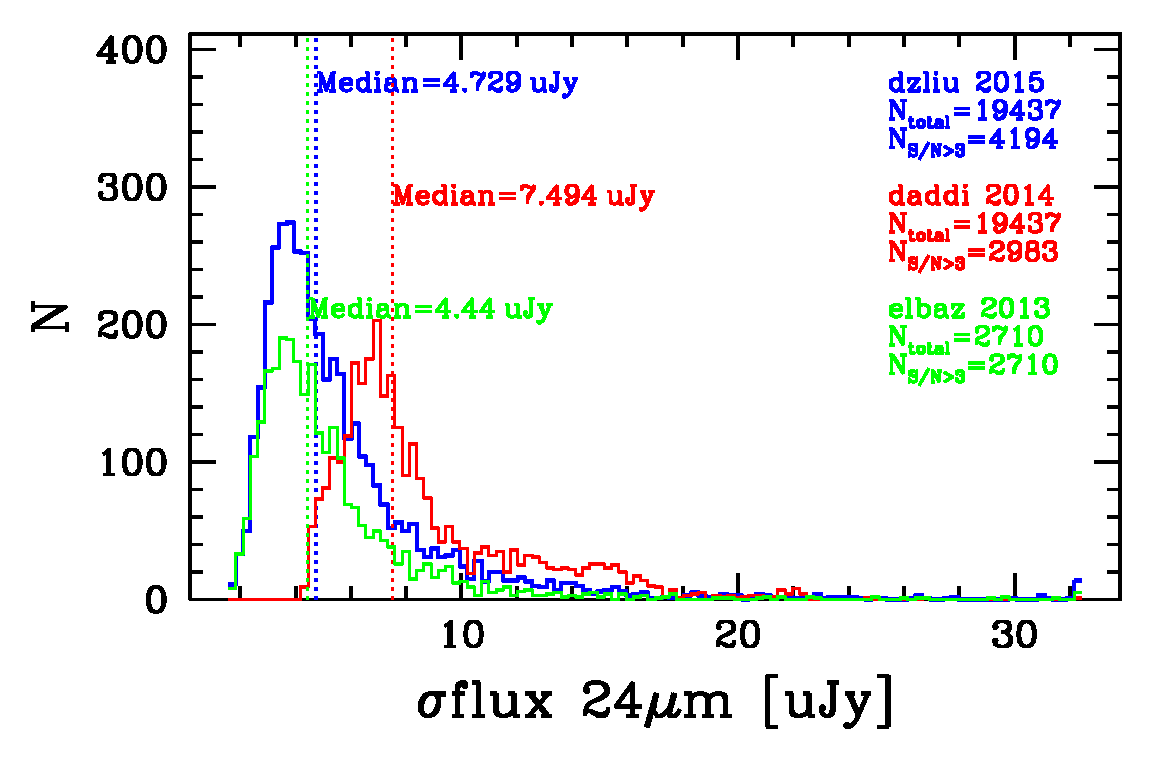
\includegraphics[width=0.75\textwidth]{compare_df24_histogram_dzliu_daddi_elbaz_20160124}
	\caption{\label{Fig_compare_f24_with_elbaz_2013}
		Comparing the new dzliu 2015 measurements with Elbaz et al. 2013 {\fontsize{7}{7}{(\url{http://adsabs.harvard.edu/abs/2013yCat..35330119E}})} measurements (the GOODS-Herschel official catalog) in the upper panel. We are showing the histogram of their flux measurements in the middle panel, and histogram of simulation-based flux errors in the bottom panel. The histograms of dzliu 2015, daddi 2014, and elbaz 2013 are shown in blue, red, and green colors respectively. }
\end{figure}

\begin{figure}[H]
	\includegraphics[width=0.75\textwidth]{compare_f24_dzliu_with_elbaz_2013_20160119}
	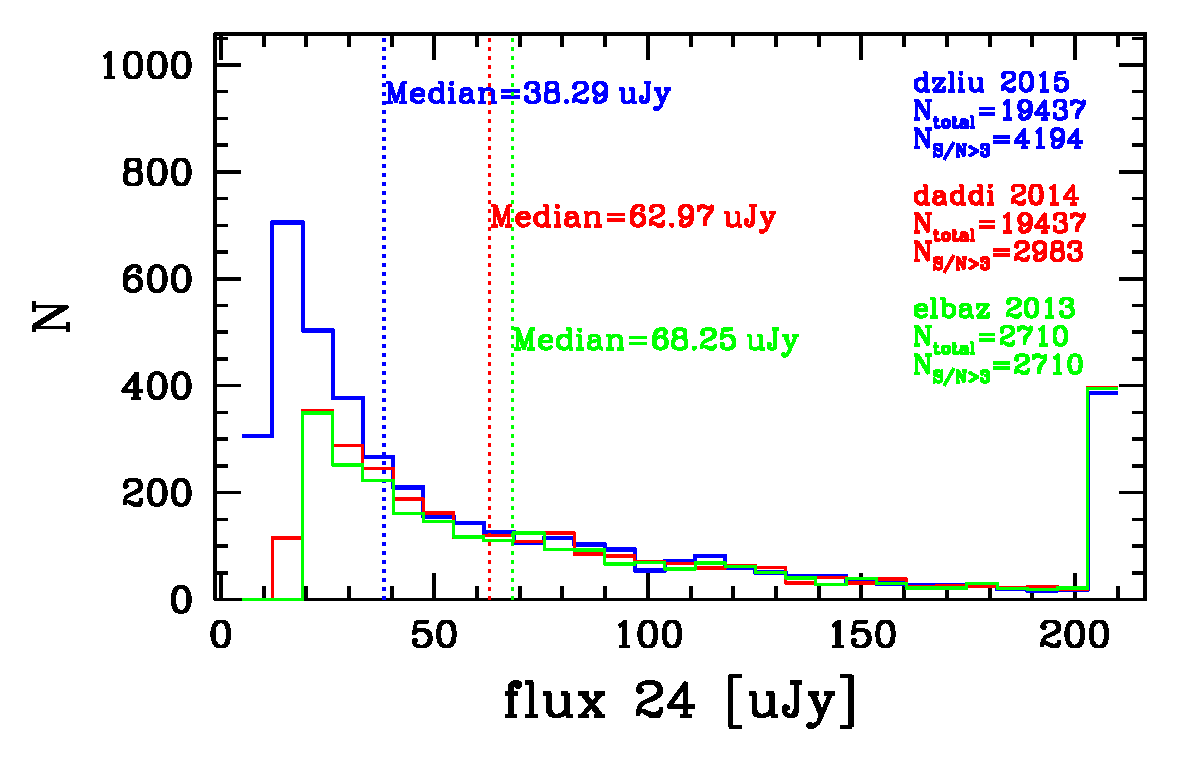
\includegraphics[width=0.75\textwidth]{compare_f24_histogram_dzliu_daddi_elbaz_20160124}
	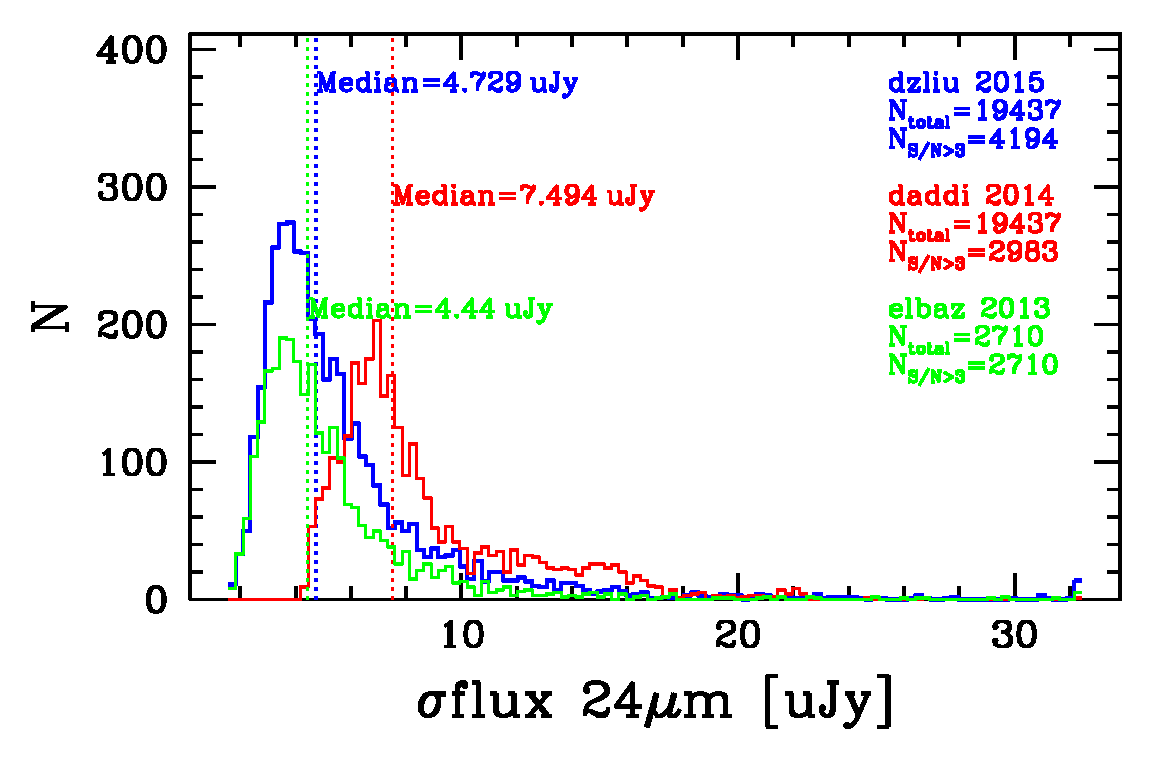
\includegraphics[width=0.75\textwidth]{compare_df24_histogram_dzliu_daddi_elbaz_20160124}
	\caption{\label{Fig_compare_df24_histogram}
		Comparing the new dzliu 2015 measurements with Elbaz et al. 2013 {\fontsize{7}{7}{(\url{http://adsabs.harvard.edu/abs/2013yCat..35330119E}})} measurements (the GOODS-Herschel official catalog) in the upper panel. We are showing the histogram of their flux measurements in the middle panel, and histogram of simulation-based flux errors in the bottom panel. The histograms of dzliu 2015, daddi 2014, and elbaz 2013 are shown in blue, red, and green colors respectively. }
\end{figure}




%*************************************************************************************

\clearpage

%*************************************************************************************
\section{Band 20cm (Owen's map)}

\subsection{Galfit at band 20cm (Owen's map)}

We use these commands to run the galfit photometry at band 20cm:

\begin{lstlisting}[language=bash]
# run first-pass without varying source position
./do_Galfit 20cm 201500 -catalog irac_mips_fluxes_hdfn.dat
cd boxgalfit; do_GalfitRunqsub; cd ..
./do_Galfit 20cm 201500 -catalog irac_mips_fluxes_hdfn.dat -postparallel
# then second-pass varying source position
./do_Galfit 20cm 201500 -catalog irac_mips_fluxes_hdfn.dat -vary
cd boxgalfit_vary; do_GalfitRunqsub; cd ..
./do_Galfit 20cm 201500 -catalog irac_mips_fluxes_hdfn.dat -vary -postparallel
\end{lstlisting}

\subsection{Galsim at band 20cm (Owen's map)}

We use these commands to run the Monte-Carlo simulation at band 20cm:

\begin{lstlisting}[language=bash]
# first estimate magnitude range
# note that 20cm 3-sigma is about 7.5uJy (Owen's map)
load astroPhot.sm
convert_flux2mag goodsn 20cm $(0.0022*01) 1 # (mBias 0 fBias -5e-05) # => 10.5112
convert_flux2mag goodsn 20cm $(0.0022*25) 1 # (mBias 0 fBias -5e-05) # => 7.03979
# then do the simulation
./do_Galsim 20cm 201500 -mag0 7.03979 -mag1 10.5112 -number 6000 -vary \
-catalog irac_mips_fluxes_hdfn.dat
cd boxgalsim; do_GalsimRunqsub; cd ..
./do_Galsim 20cm 201500 -mag0 7.03979 -mag1 10.5112 -number 6000 -vary \
-catalog irac_mips_fluxes_hdfn.dat -postparallel
\end{lstlisting}

\subsection{Galsim Analysis at band 20cm (Owen's map)}

We use these commands to run the simulation analysis at band 20cm:

\begin{lstlisting}[language=bash]
cd doing20cm/
sm
macro read run_simu_stats_v7.sm run_simu_stats_v7 20cm 201500
\end{lstlisting}

Below are our statistical analyses:

\begin{figure}[H]
	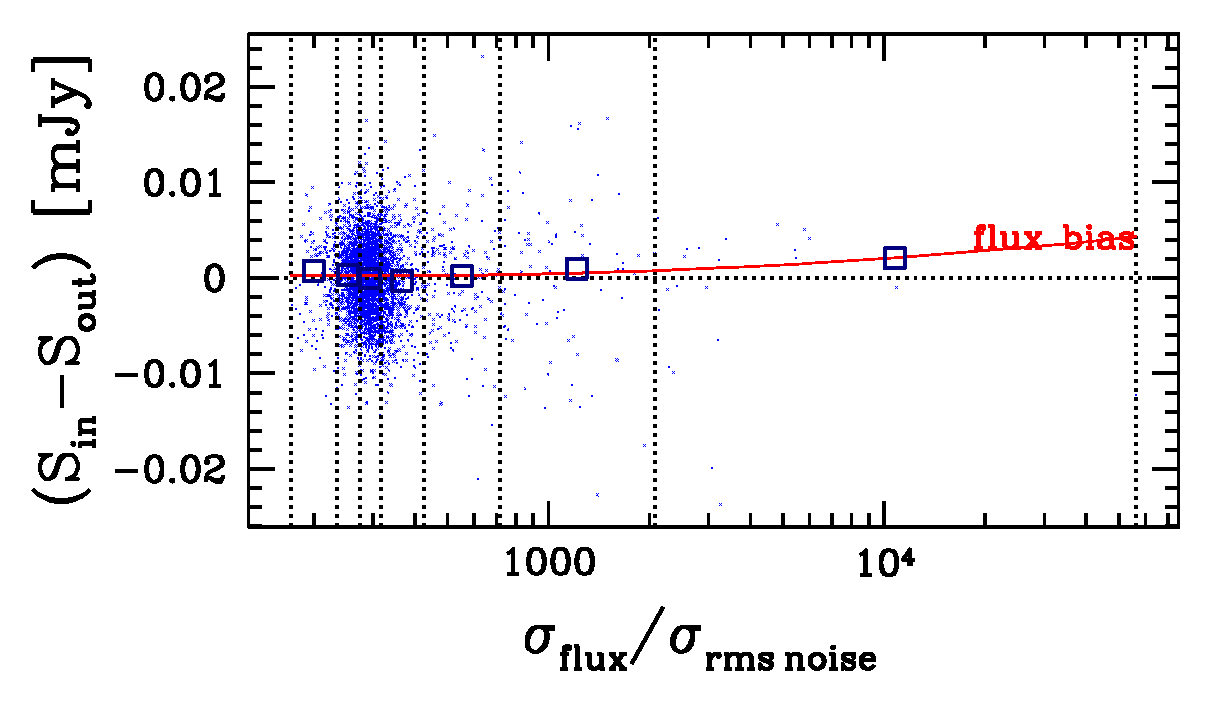
\includegraphics[width=0.8\textwidth]{galsim_20cm_fbias_1}
	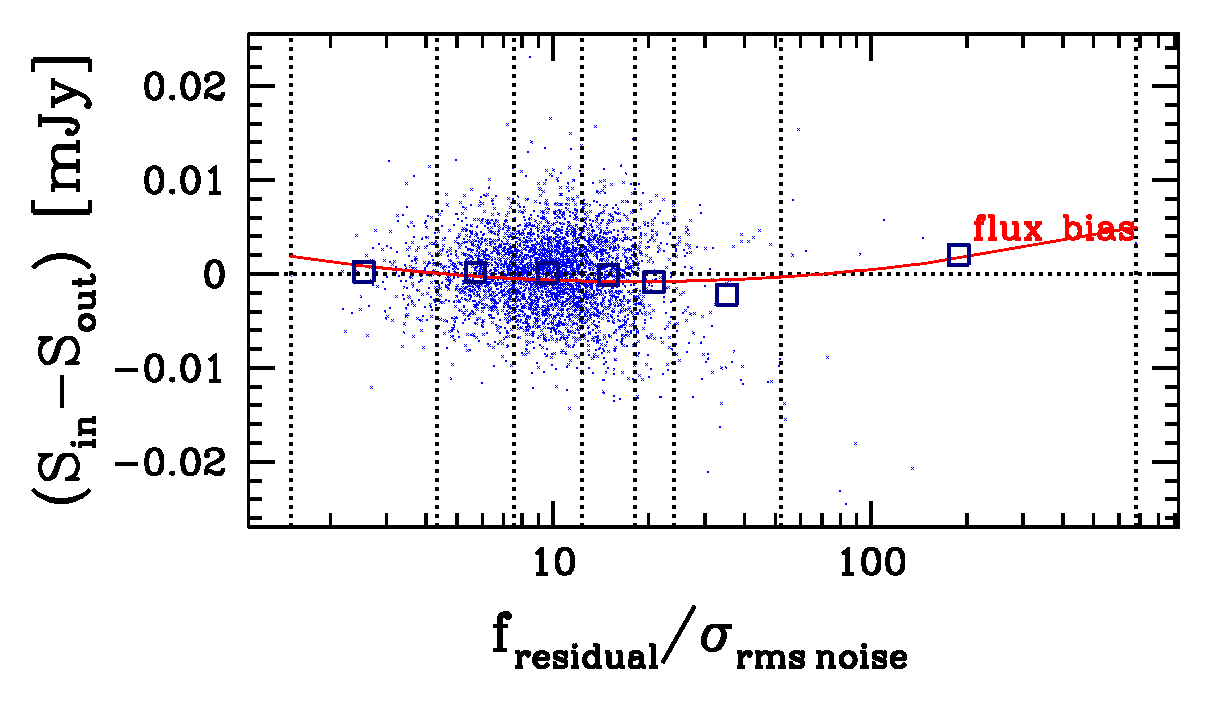
\includegraphics[width=0.8\textwidth]{galsim_20cm_fbias_2}
	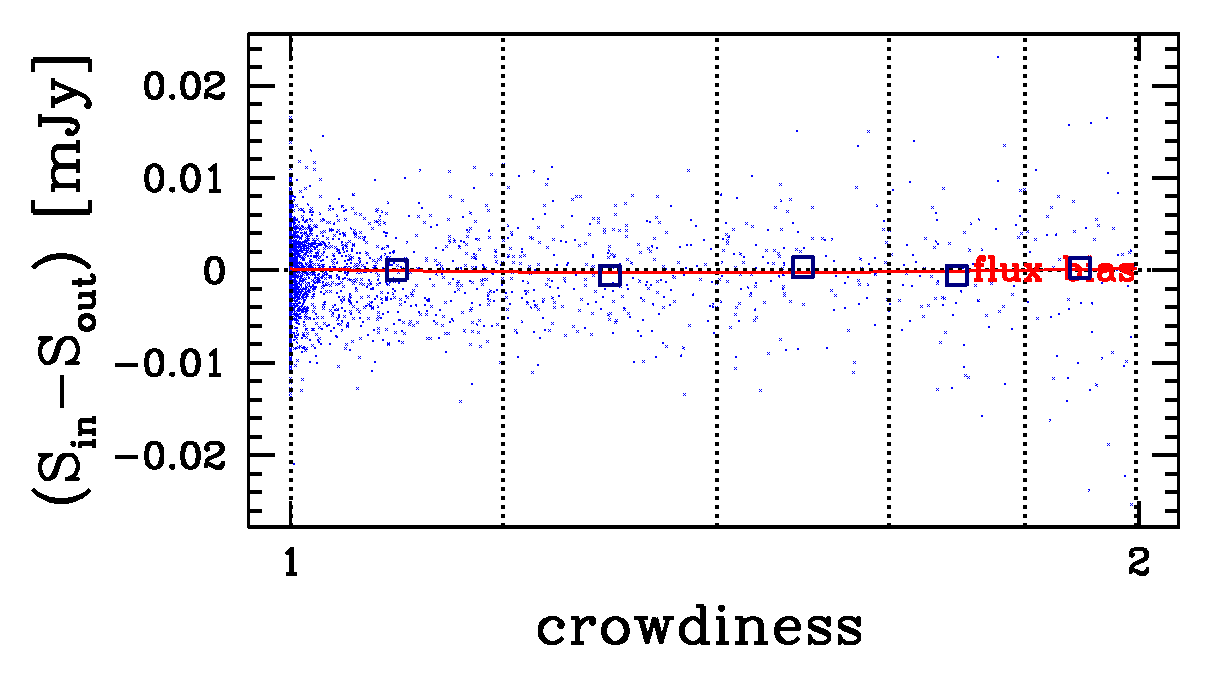
\includegraphics[width=0.8\textwidth]{galsim_20cm_fbias_3}
	\caption{Flux bias analysis from simulation.}
\end{figure}

\begin{figure}[H]
	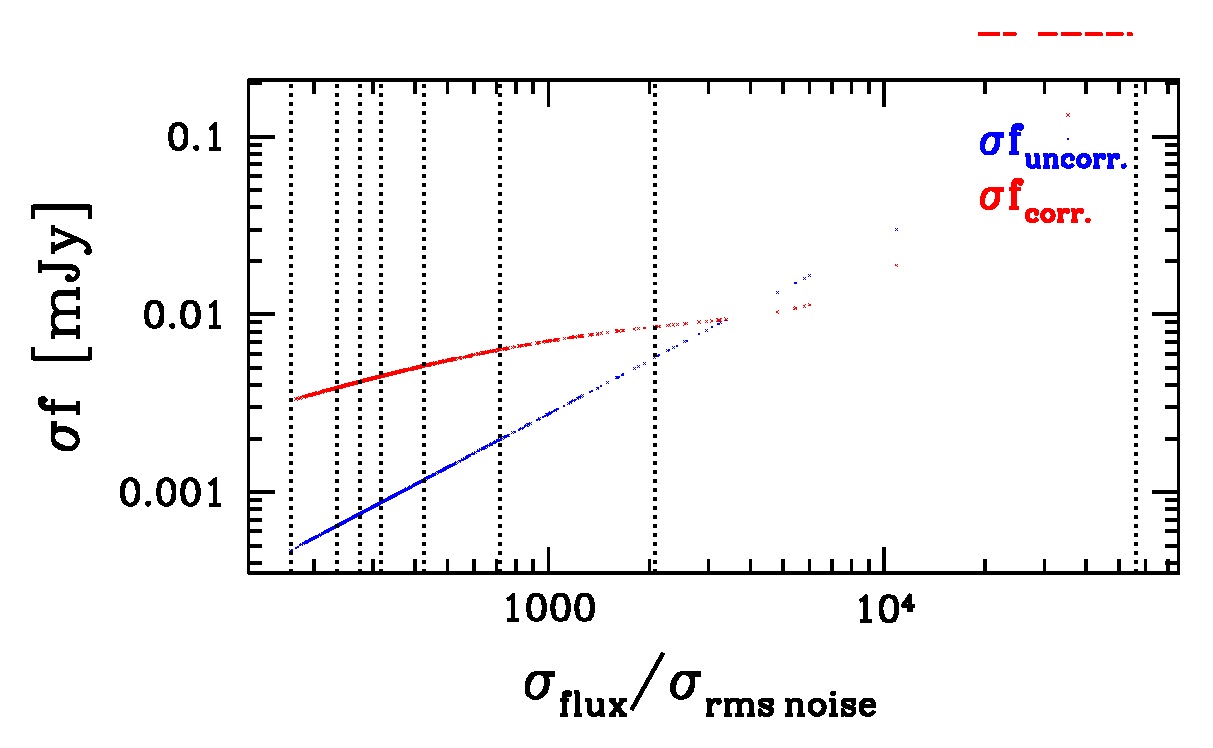
\includegraphics[width=0.8\textwidth]{galsim_20cm_dfcorr_1}
	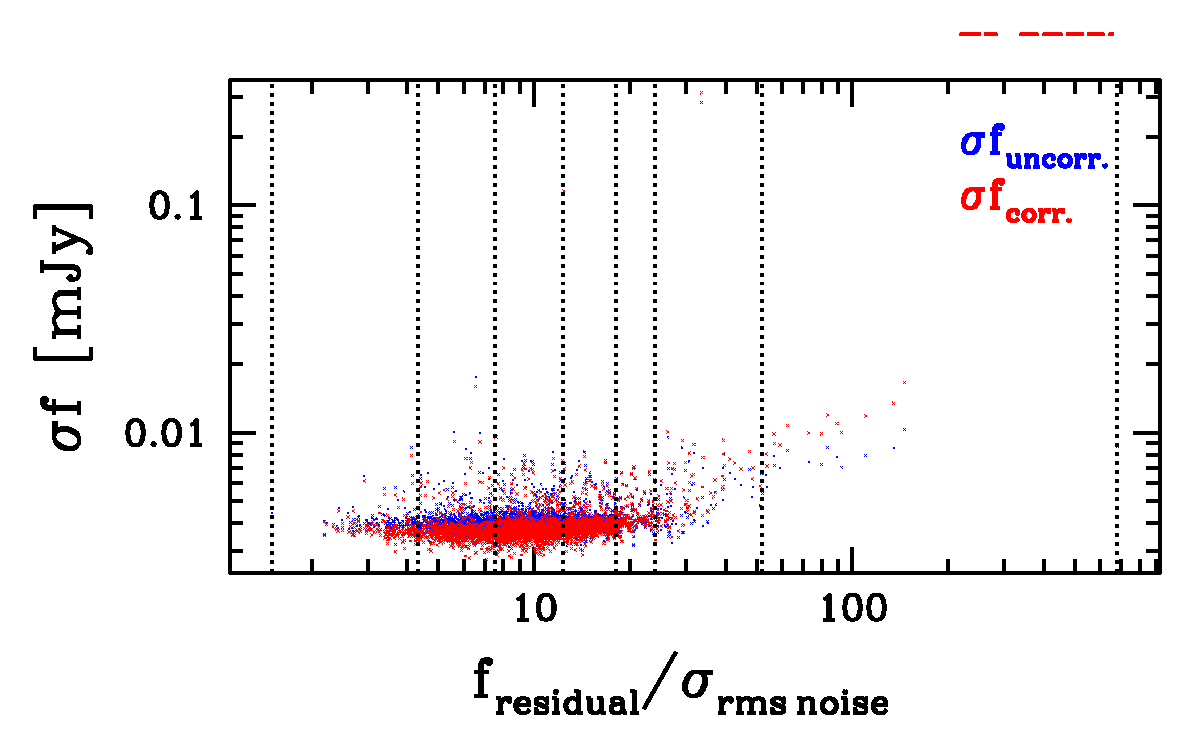
\includegraphics[width=0.8\textwidth]{galsim_20cm_dfcorr_2}
	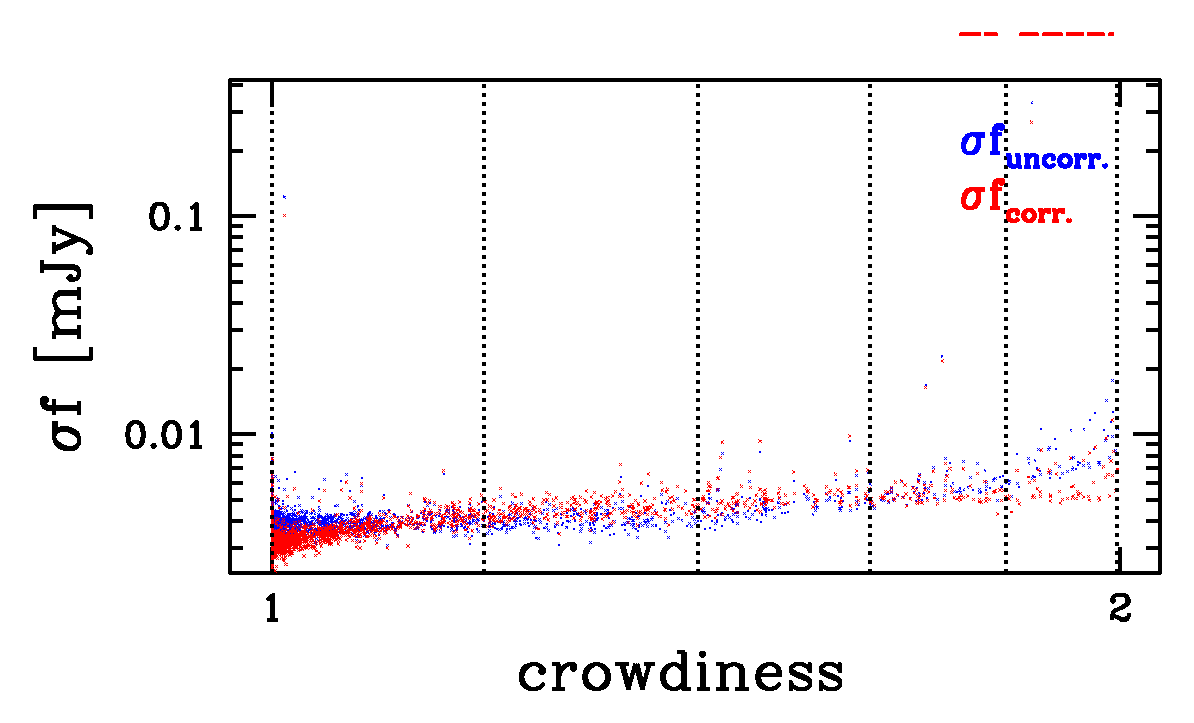
\includegraphics[width=0.8\textwidth]{galsim_20cm_dfcorr_3}
	\caption{Flux uncertainty analysis from simulation.}
\end{figure}

\begin{figure}[H]
	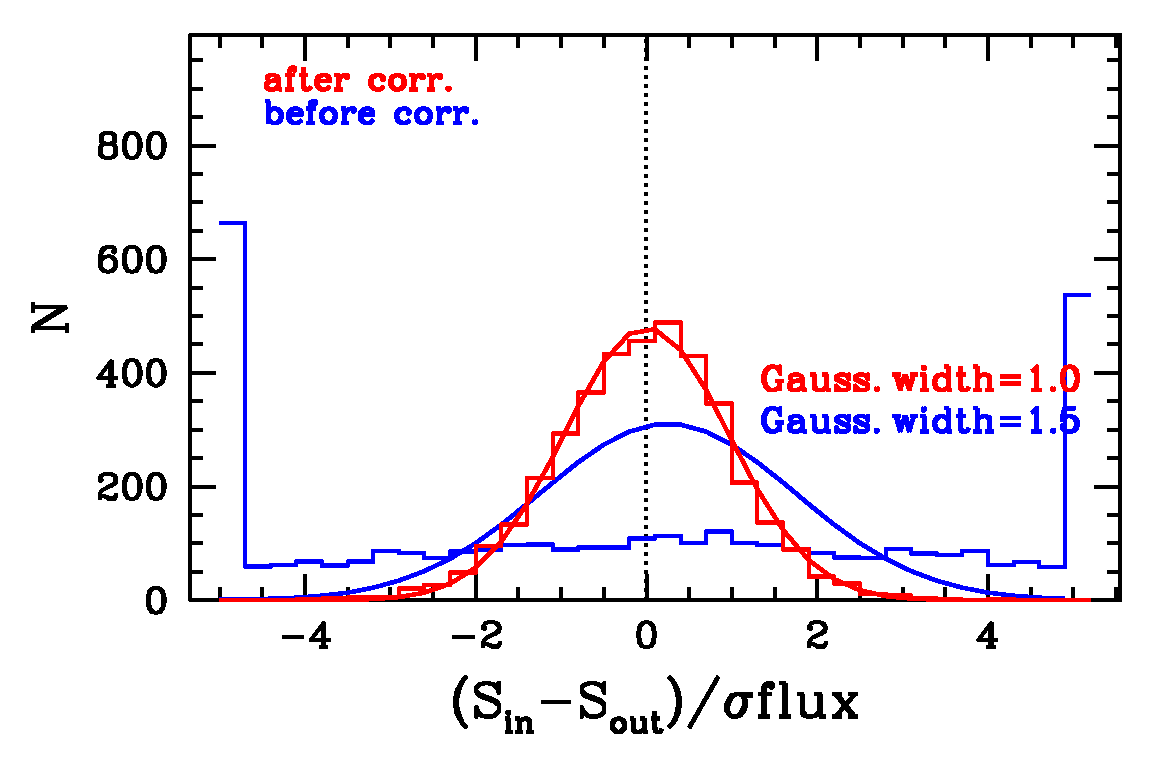
\includegraphics[width=0.75\textwidth]{galsim_20cm_hist_dfcorr_1}
	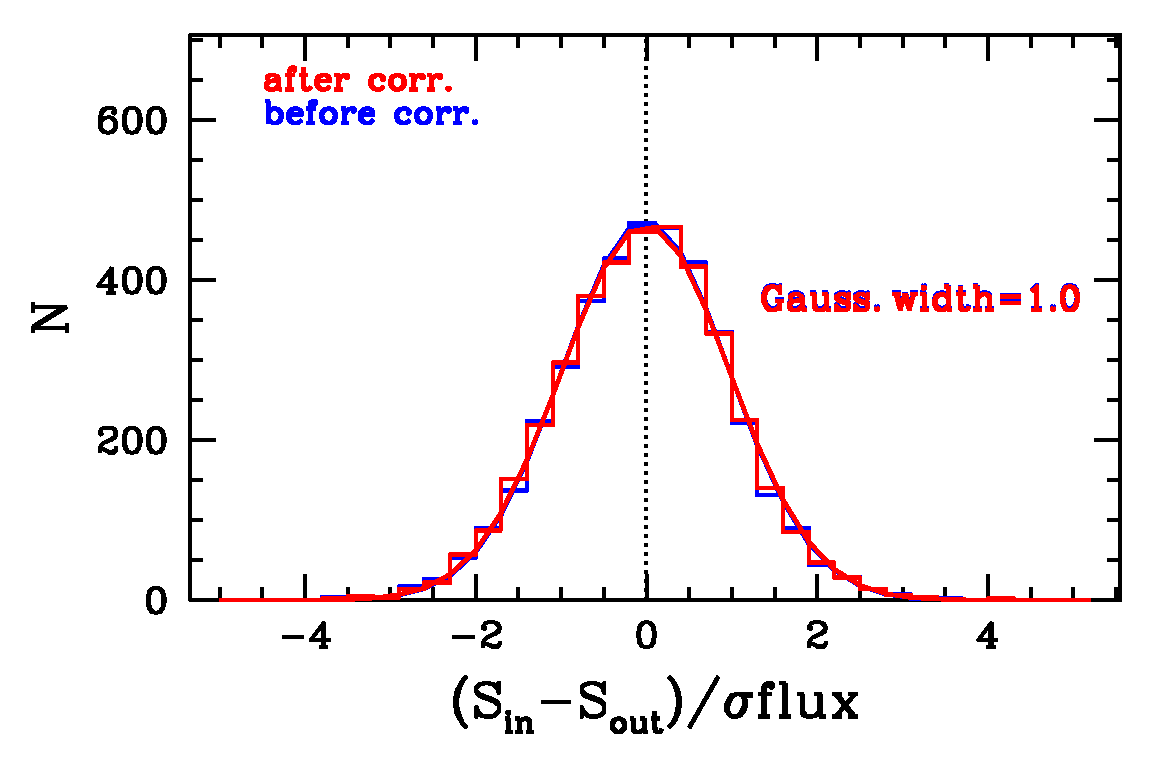
\includegraphics[width=0.75\textwidth]{galsim_20cm_hist_dfcorr_2}
	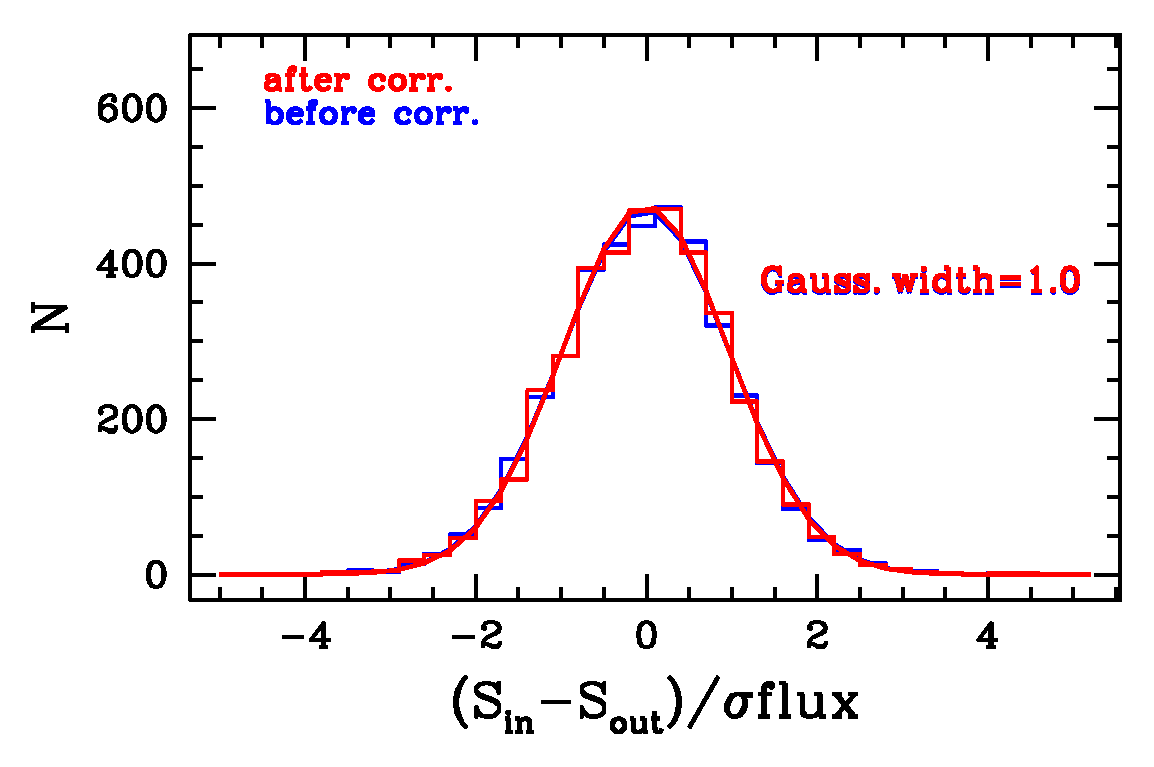
\includegraphics[width=0.75\textwidth]{galsim_20cm_hist_dfcorr_3}
	\caption{Statistical behavior of input minus output differences before and after correction.}
\end{figure}

\subsection{Compare with literature: Elbaz et al. 2013}

\begin{figure}[H]
	\includegraphics[width=0.95\textwidth]{compare_f24_dzliu_with_elbaz_2013_20160119}
	\caption{Compare our final corrected 24${\mu}m$ measurements with the literature measurements of Elbaz et al. 2013 (\fontsize{8}{8}{\url{http://adsabs.harvard.edu/abs/2013yCat..35330119E}}). Y axis is our measurements. A linear dashed green-black line indicates a one-to-one correlation. Details of the most outliers are given below: ID11828 is bright and extended, our PSF fitting could not recover its entire flux. ID13543 is bright and blended with its neighborhood ID13542 which is also bright. Not sure why and how to fix yet \textcolor{red}{(TODO)}. ID3159 and ID3119 are close within 2'' and the peak of flux at in between of them. ID10754 is only 15'' from the bright 20'' diameter spiral source ID10611, therefore got highly contaminated results. ID18254 and ID18253 are blended, and the latter one is brighter and likely extended, hence the former one got contaminated flux.}
\end{figure}

%*************************************************************************************

\clearpage

%*************************************************************************************
\section{Band 20cm (Morrison's map)}

\subsection{Galfit at band 20cm (Morrison's map)}

We use these commands to run the galfit photometry at band 20cm:

\begin{lstlisting}[language=bash]
# run first-pass without varying source position
./do_Galfit 20cm_Glenn 201500 -catalog irac_mips_fluxes_hdfn.dat
cd boxgalfit; do_GalfitRunqsub; cd ..
./do_Galfit 20cm_Glenn 201500 -catalog irac_mips_fluxes_hdfn.dat -postparallel
# then second-pass varying source position
./do_Galfit 20cm_Glenn 201500 -catalog irac_mips_fluxes_hdfn.dat -vary
cd boxgalfit_vary; do_GalfitRunqsub; cd ..
./do_Galfit 20cm_Glenn 201500 -catalog irac_mips_fluxes_hdfn.dat -vary -postparallel
\end{lstlisting}

\subsection{Galsim at band 20cm (Morrison's map)}

We use these commands to run the Monte-Carlo simulation at band 20cm:

\begin{lstlisting}[language=bash]
# first estimate magnitude range
# In Morrison et al. 2010 catalog, 1230 radio sources were detected. 
# Their median df20cm is ~10uJy, while minimum df20cm is ~3uJy. 
# Their minimum f20cm is ~21uJy, and maximum f20cm is ~263uJy. 
# Therefore we do simulation with f20cm from 10uJy to 263uJy. 
load astroPhot.sm
convert_flux2mag goodsn 20cm_Glenn 0.010 1 # (mBias 0 fBias 0) # => 9.6961
convert_flux2mag goodsn 20cm_Glenn 0.263 1 # (mBias 0 fBias 0) # => 6.14621
# then do the simulation
./do_Galsim 20cm_Glenn 201500 -mag0 6.14621 -mag1 9.6961 -number 6000 -vary \
-catalog irac_mips_fluxes_hdfn.dat
cd boxgalsim; do_GalsimRunqsub; cd ..
./do_Galsim 20cm_Glenn 201500 -mag0 6.14621 -mag1 9.6961 -number 6000 -vary \
-catalog irac_mips_fluxes_hdfn.dat -postparallel
\end{lstlisting}

The above simulations have too many bright sources. A faint end $\sim10{\mu}Jy$ the behaviors are not well understood. Therefore we run fainter simulations below. 

\begin{lstlisting}[language=bash]
# first estimate magnitude range
# In Morrison et al. 2010 catalog, 1230 radio sources were detected. 
# Their median df20cm is ~10uJy, while minimum df20cm is ~3uJy. 
# Their minimum f20cm is ~21uJy, and maximum f20cm is ~263uJy. 
# Therefore we do simulation with f20cm from 10uJy to 263uJy. 
load astroPhot.sm
convert_flux2mag goodsn 20cm_Glenn $(0.0022*01) 1 # (mBias 0 fBias 0) # => 11.34
convert_flux2mag goodsn 20cm_Glenn $(0.0022*25) 1 # (mBias 0 fBias 0) # => 7.84519
# then do the simulation
./do_Galsim 20cm_Glenn 20160115 -mag0 7.84519 -mag1 11.34 -number 6000 -vary \
-catalog irac_mips_fluxes_hdfn.dat
cd boxgalsim; do_GalsimRunqsub; cd ..
./do_Galsim 20cm_Glenn 20160115 -mag0 7.84519 -mag1 11.34 -number 6000 -vary \
-catalog irac_mips_fluxes_hdfn.dat -postparallel
\end{lstlisting}

\subsection{Galsim Analysis at band 20cm (Morrison's map)}

We use these commands to run the simulation analysis at band 20cm:

\begin{lstlisting}[language=bash]
cd doing20cm_Glenn/
sm
macro read run_simu_stats_v7.sm run_simu_stats_v7 20cm_Glenn 201500
\end{lstlisting}

Below are our statistical analyses:

\begin{figure}[H]
	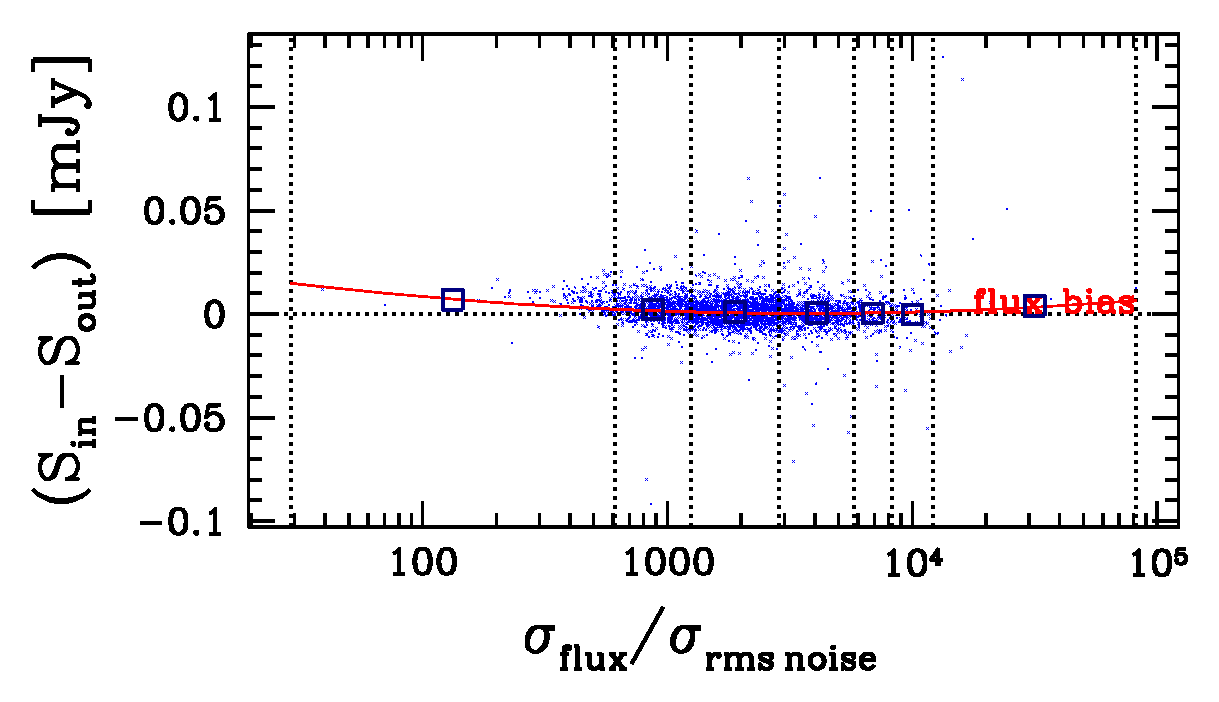
\includegraphics[width=0.8\textwidth]{galsim_20cm_Glenn_fbias_1}
	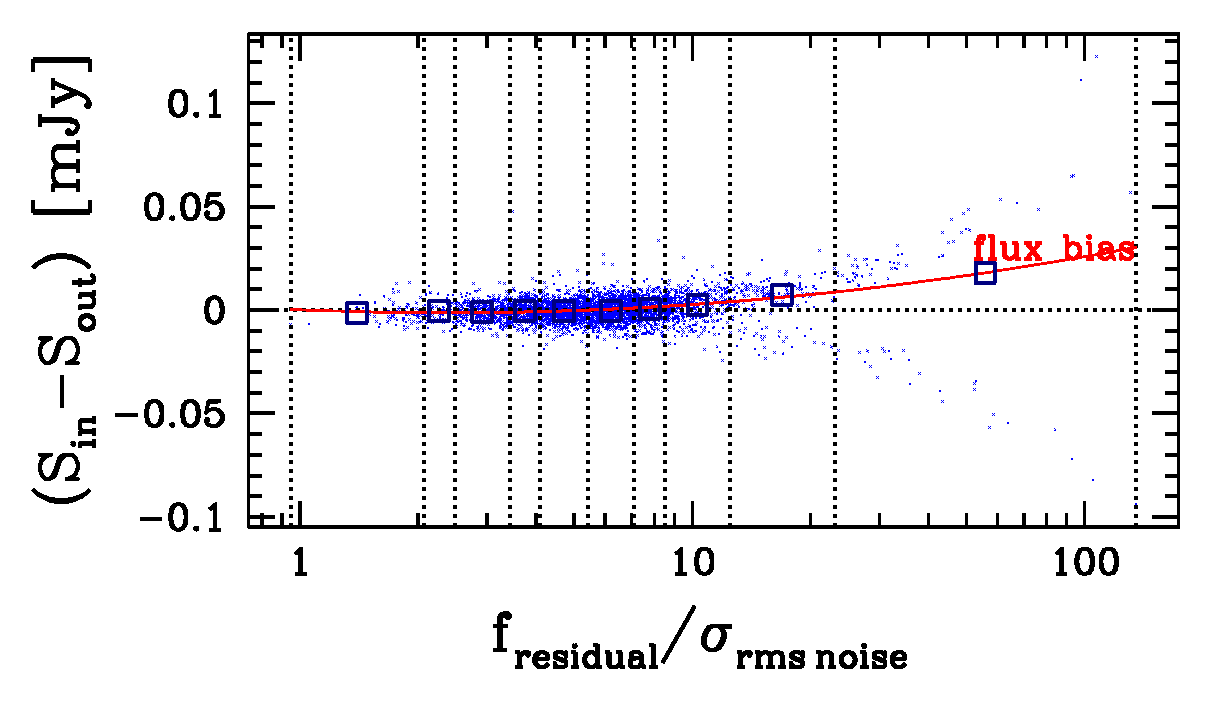
\includegraphics[width=0.8\textwidth]{galsim_20cm_Glenn_fbias_2}
	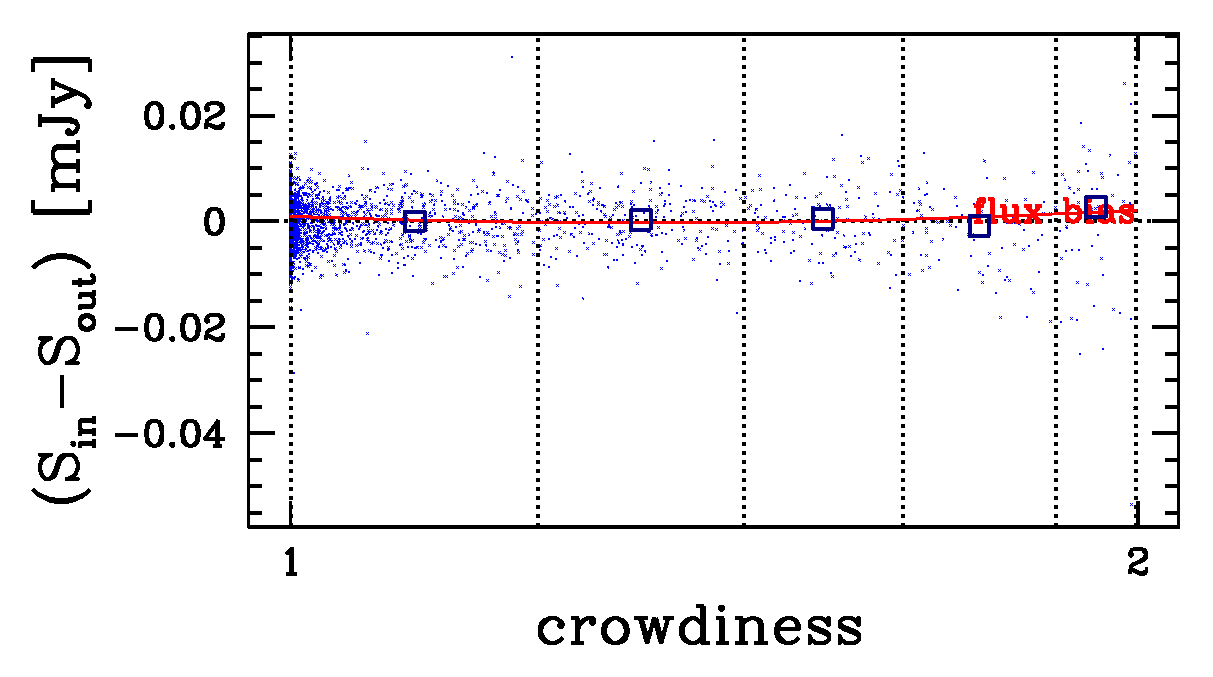
\includegraphics[width=0.8\textwidth]{galsim_20cm_Glenn_fbias_3}
	\caption{Flux bias analysis from simulation.}
\end{figure}

\begin{figure}[H]
	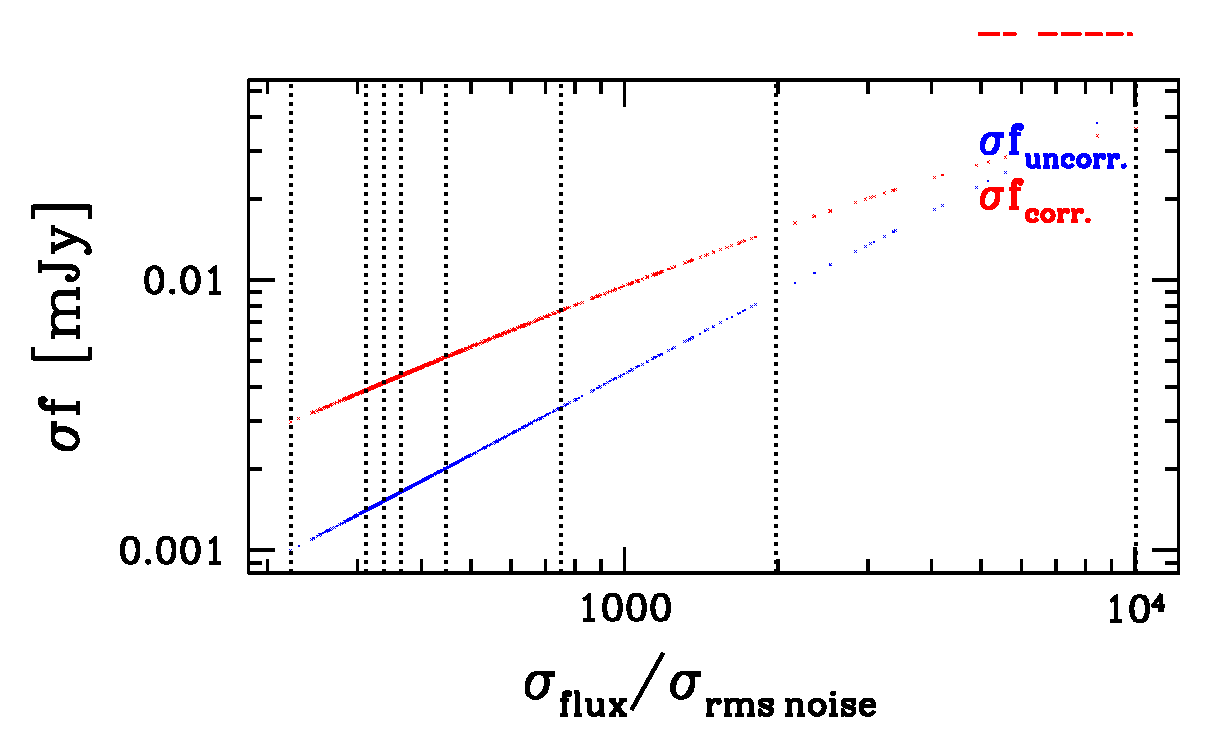
\includegraphics[width=0.8\textwidth]{galsim_20cm_Glenn_dfcorr_1}
	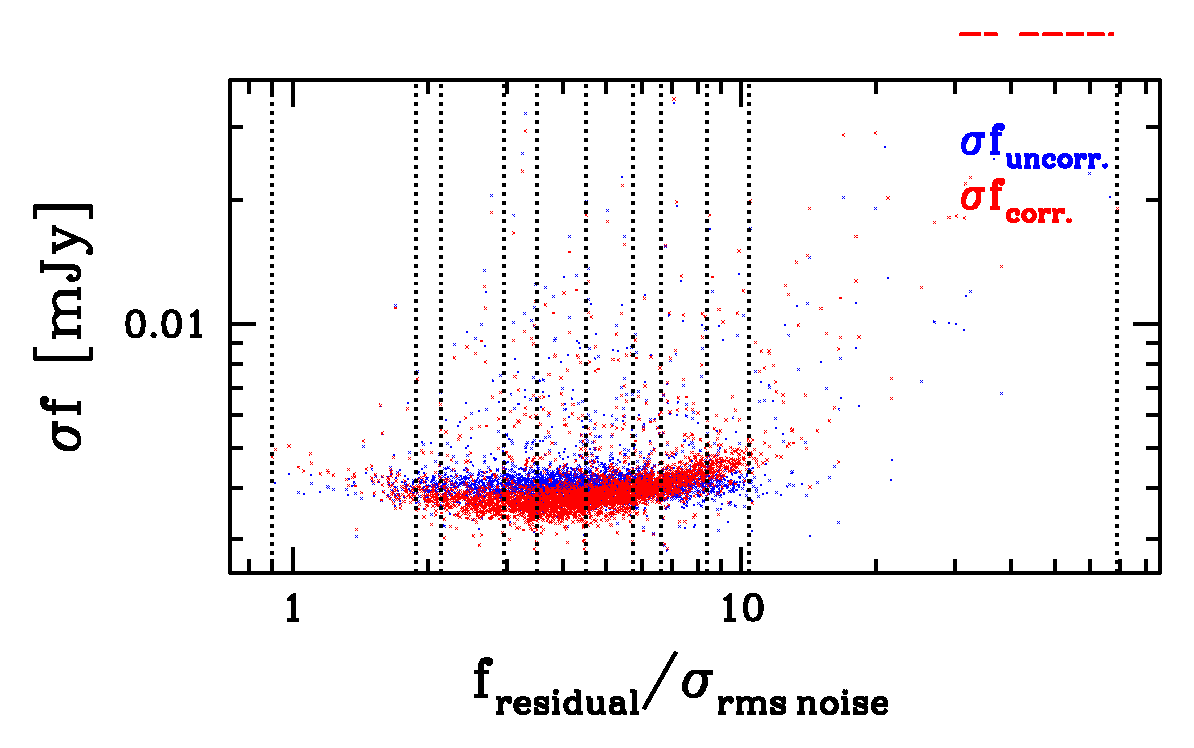
\includegraphics[width=0.8\textwidth]{galsim_20cm_Glenn_dfcorr_2}
	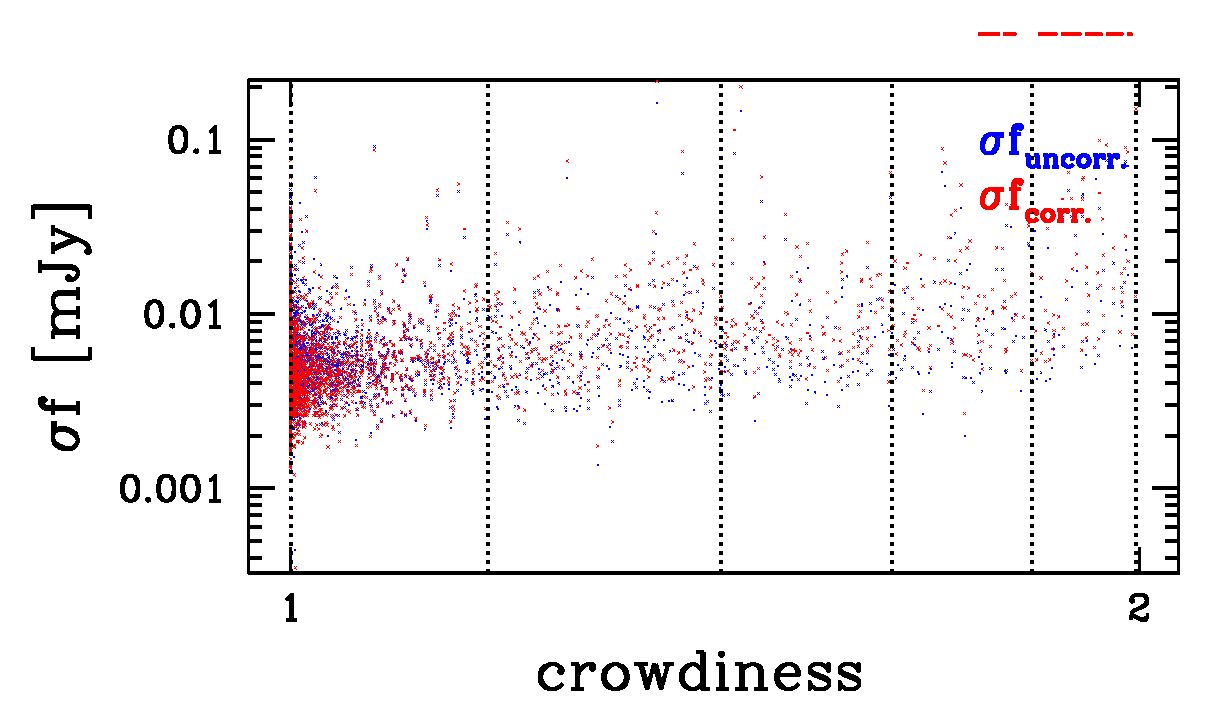
\includegraphics[width=0.8\textwidth]{galsim_20cm_Glenn_dfcorr_3}
	\caption{Flux uncertainty analysis from simulation.}
\end{figure}

\begin{figure}[H]
	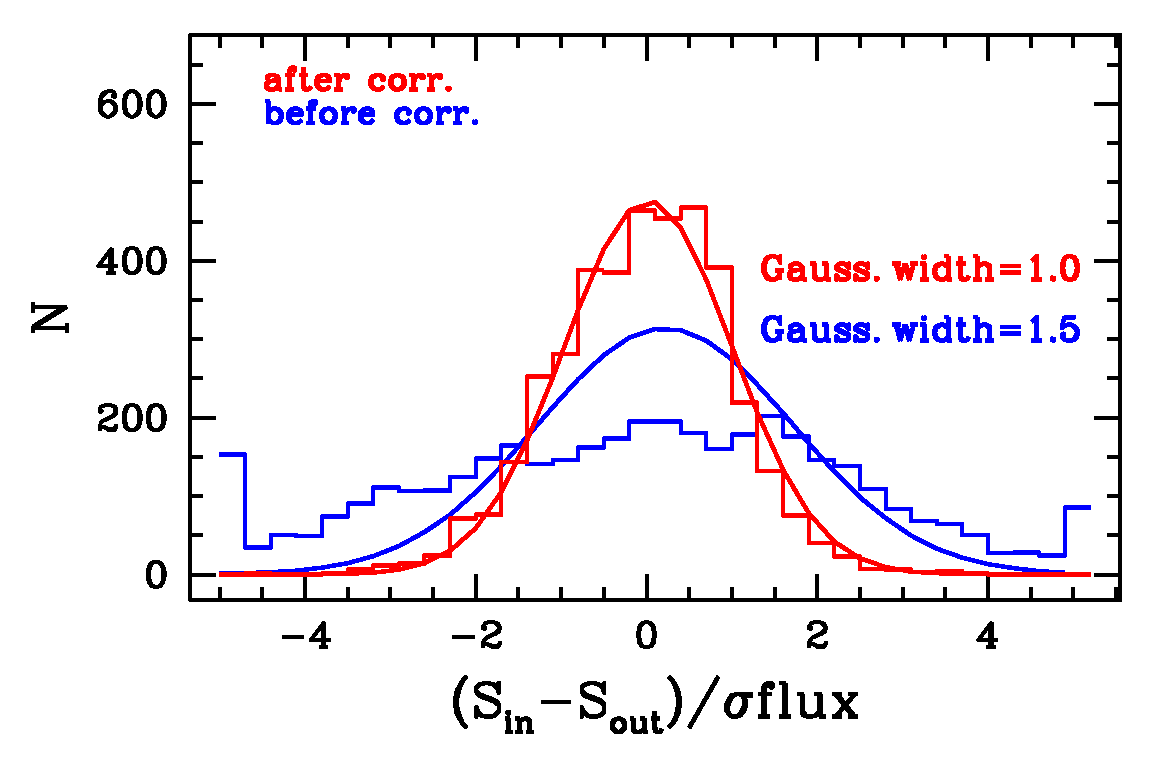
\includegraphics[width=0.75\textwidth]{galsim_20cm_Glenn_hist_dfcorr_1}
	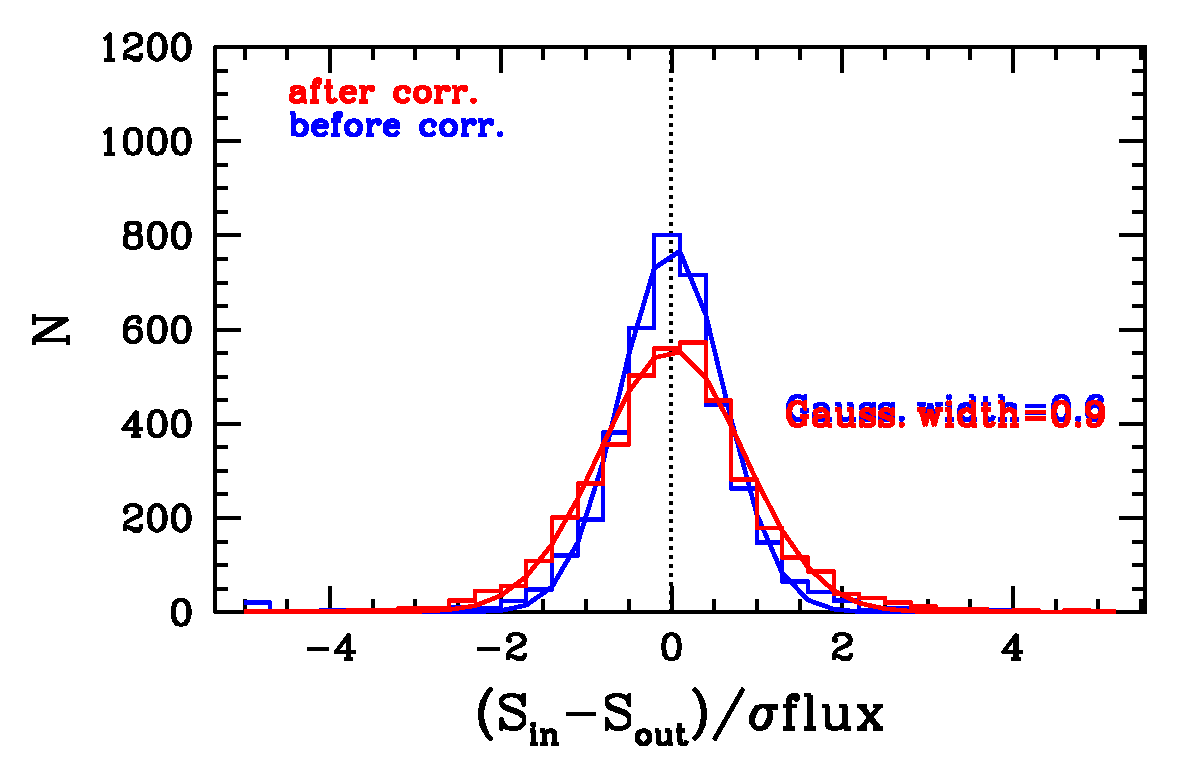
\includegraphics[width=0.75\textwidth]{galsim_20cm_Glenn_hist_dfcorr_2}
	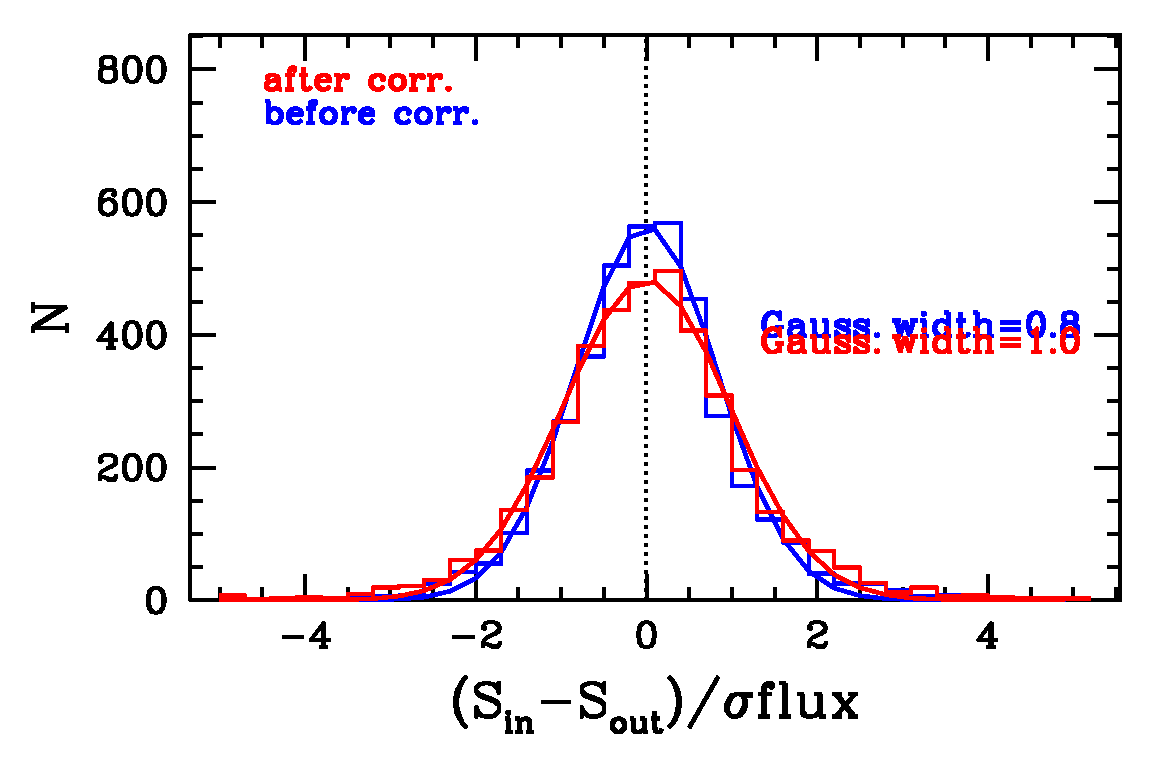
\includegraphics[width=0.75\textwidth]{galsim_20cm_Glenn_hist_dfcorr_3}
	\caption{\label{galsim_20cm_Glenn_hist}
		Statistical behavior of input minus output differences before and after correction.}
\end{figure}

\subsection{Compare with literature: Morrison et al. 2010}

\begin{figure}[H]
	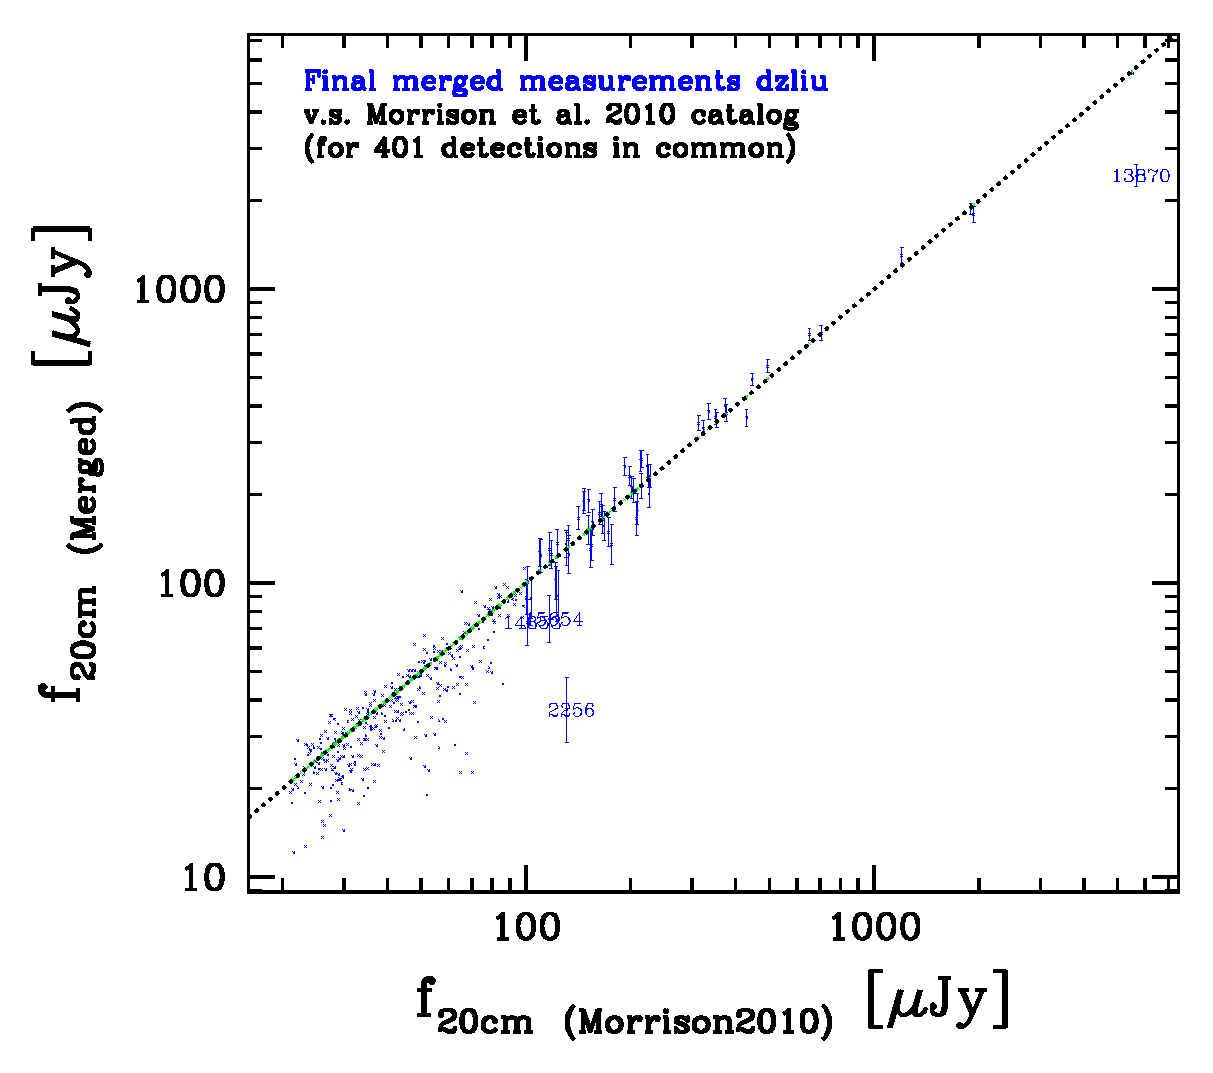
\includegraphics[width=0.95\textwidth]{compare_f20cm_dzliu_with_morrison_2010_20160119}
	\caption{Comparing dzliu 2015 two-radio-map-merged and sim-recipe-corrected 20cm measurements with the literature measurements in Morrison et al. 2010. Y axis is our measurements. A linear dashed black line indicates a one-to-one correlation. Details of several obvious outliers: ID13870 is an extremely bright radio source and has two peaks, likely two interacting components? ID2256 is relatively bright but heavily extended, and what we are fitting is PSF for now, hence could not recover its entire flux.}
\end{figure}

\begin{figure}[H]
	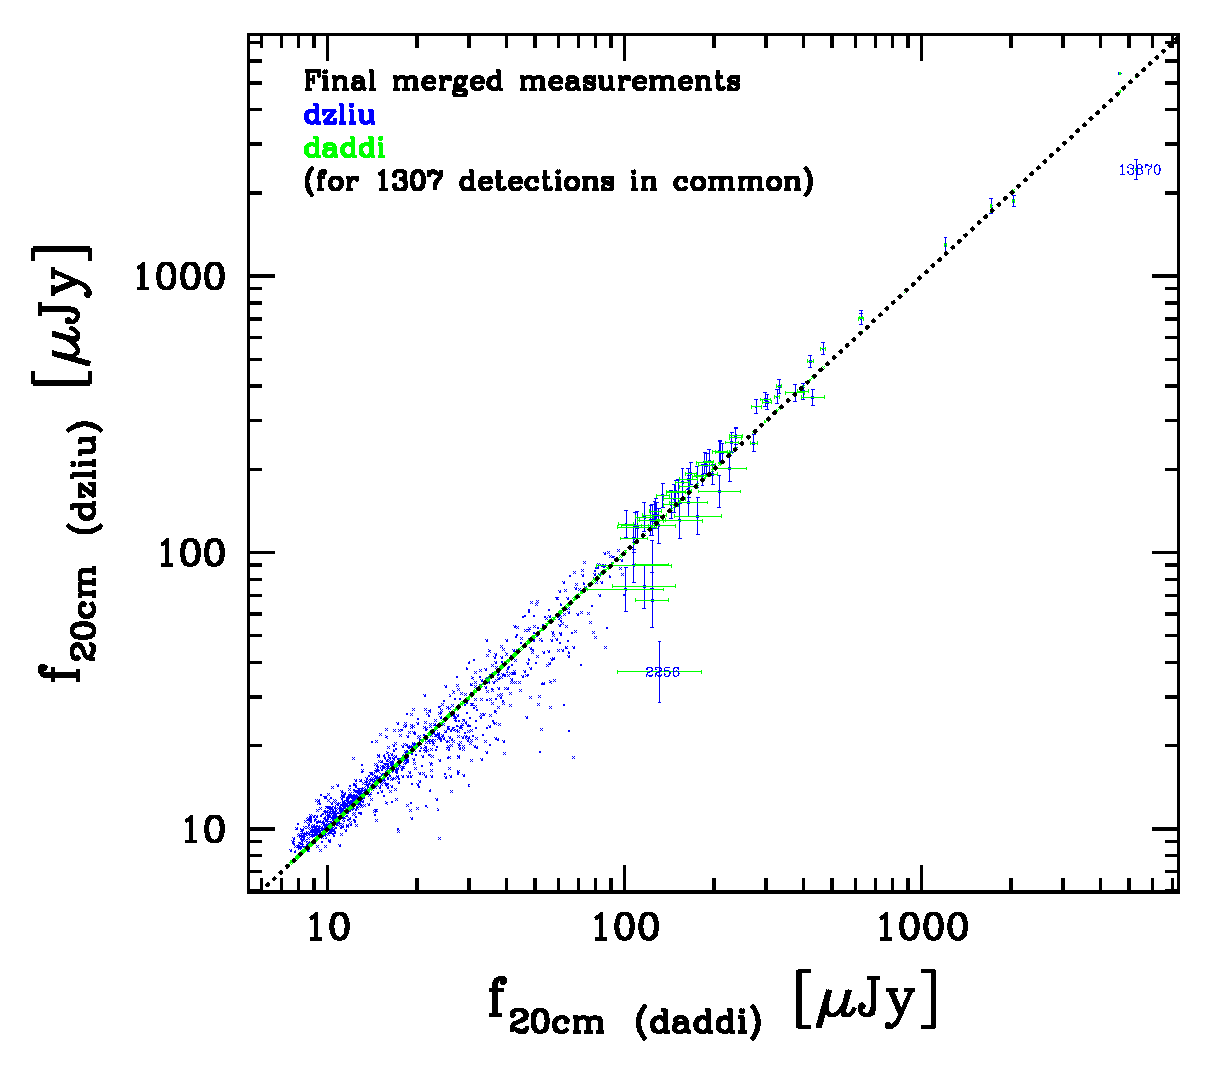
\includegraphics[width=0.95\textwidth]{compare_f20cm_dzliu_with_daddi_20160119}
	\caption{Comparing dzliu 2015 measurements with our previous work daddi 2014 measurements. Y axis is dzliu 2015 measurements and X axis is daddi 2014 measurements. A linear dashed black line indicates a one-to-one correlation. Vertical black error bars are dzliu 2015 flux errors, and horizontal green error bars are daddi 2014 flux errors.}
\end{figure}

\begin{figure}[H]
	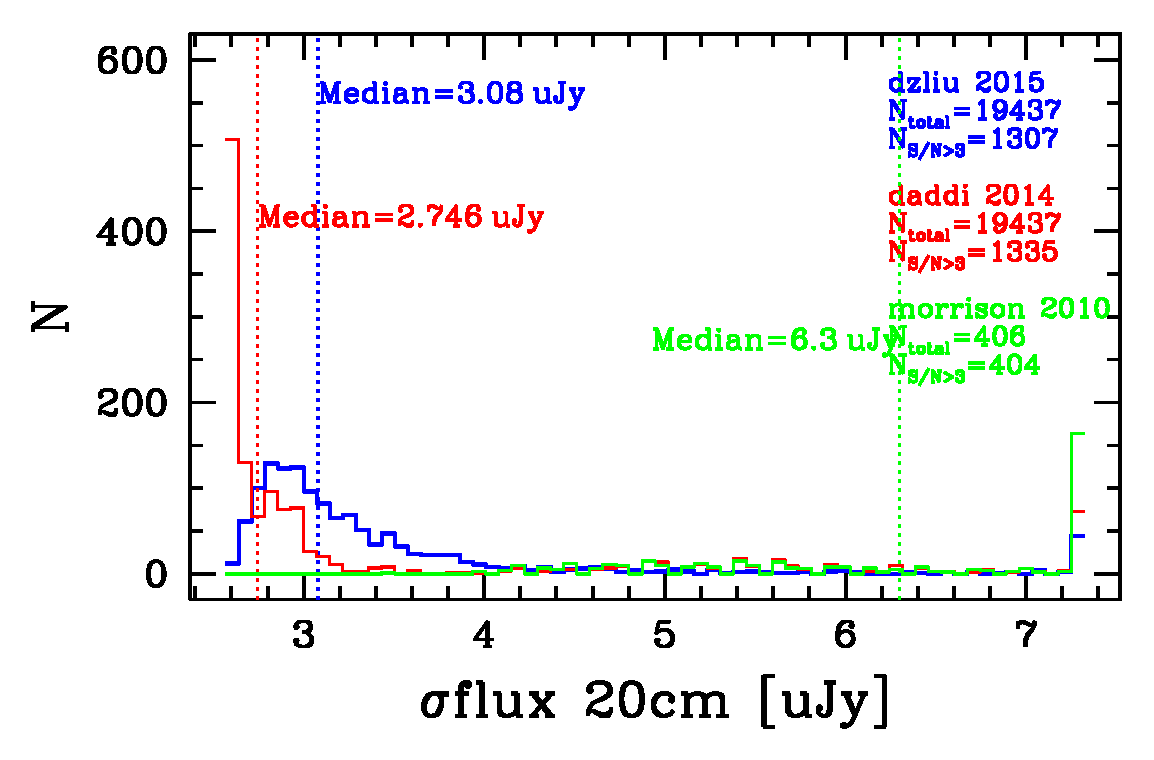
\includegraphics[width=0.95\textwidth]{compare_df20cm_histogram_dzliu_daddi_morrison_20160124}
	\caption{Comparing the histograms of 3 flux errors: dzliu 2015, which have applied simulation-based correction recipes to flux biases and flux errors; daddi 2014, which are previous results but have higher reliability; morrison 2010, which are published results and are the flux errors derived from uv data, but have much fewer sources.}
\end{figure}

\begin{figure}[H]
	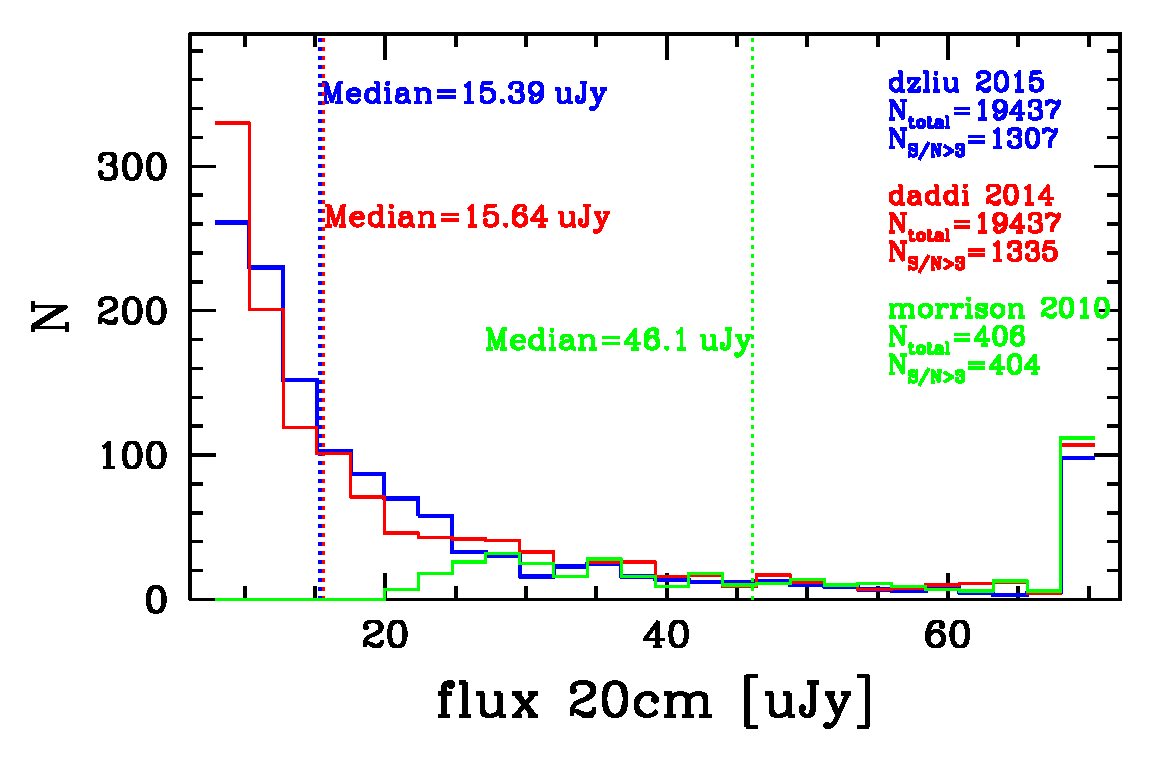
\includegraphics[width=0.95\textwidth]{compare_f20cm_histogram_dzliu_daddi_morrison_20160124}
	\caption{Comparing the histograms of 3 flux measurements: dzliu 2015, which have applied simulation-based correction recipes to flux biases and flux errors; daddi 2014, which are previous results but have higher reliability; morrison 2010, which are published results and are the flux errors derived from uv data, but have much fewer sources.}
\end{figure}

%*************************************************************************************

\clearpage

%*************************************************************************************

\section{Selecting 24+radio source}

%*************************************************************************************

\clearpage

%*************************************************************************************

\section{Band 16}
\subsection{Galsim at band 24}

We use these commands to run the Monte-Carlo simulation at band 24:

\begin{lstlisting}[language=bash]
sm
load astroPhot.sm # `{\color{gray}\fontsize{5}{5}{\url{https://github.com/1054/DeepFields.SuperDeblending/blob/master/Softwares/Supermongo_macro/astroPhot.sm}}}`
# first estimate magnitude range
convert_flux2mag goodsn 16 $(0.005*01) 1 # 1.45117
convert_flux2mag goodsn 16 $(0.005*50) 1 # -2.79625
# then do the simulation
./do_Galsim 16 201500 -mag0 -2.79625 -mag1 1.45117 -number 6000 \
-catalog RadioOwenMIPS24_priors_April18_2014.txt \
-fitsname goods_north_wdriz_frac0pt6_norm_19dec06_subbackDL.fits
cd boxgalsim; do_GalsimRunqsub; cd ..
./do_Galsim 16 201500 -mag0 -3.5 -mag1 0.0 -number 6000 \
-catalog RadioOwenMIPS24_priors_April18_2014.txt \
-fitsname goods_north_wdriz_frac0pt6_norm_19dec06_subbackDL.fits -postparallel
\end{lstlisting}

\subsection{Galsim Analysis at band 16}

We use these commands to run the simulation analysis at band 16:

\begin{lstlisting}[language=bash]
sm
macro read run_simu_stats_v7.sm run_simu_stats_v7 16 201500
\end{lstlisting}

%*************************************************************************************

\clearpage

%*************************************************************************************
\appendix

%*************************************************************************************
\section{Software Dependencies}
\label{Appendix_Software_Dependencies}

\begin{lstlisting}[language=bash]
supermongo
BASH
IRAF
galfit
wcstools # http://tdc-www.harvard.edu/software/wcstools/wcstools-3.9.2.tar.gz
CrabPhotAperPhot # for measuring aperture photometry on residual image. TODO: github url
CrabTableReadColumn # for reading fixed width ascii table
\end{lstlisting}

%*************************************************************************************

\clearpage

%*************************************************************************************
\section{Discussed Issues}
\label{Appendix_DiscussedIssues}

\subsection{Do we use dzliu 2015 24${\mu}m$ measurements?}

\textcolor{green!90!black!60!orange}{Date: 2016-01-20 02:41 AM UTC+8}

Perhaps yes. The simulation-based 3-step correction recipes work well (e.g. Figure \ref{galsim_20cm_Glenn_hist}). 

\subsection{Do we use dzliu 2015 20$cm$ measurements?}

\textcolor{green!90!black!60!orange}{Date: 2016-01-20 02:41 AM UTC+8}

Perhaps no. For the radio the beam (PSF) is so small that the 3-step correction recipes, which involve crowdiness (i.e. number of sources per Gaussian beam) and residual flux might not work. So stick to previous stable old measurements. 

\subsection{How are dzliu 2015 24${\mu}m$ measurements affecting 24+radio catalog selection?}

\textcolor{green!90!black!60!orange}{Date: 2016-01-20 07:45 PM UTC+8}

It seems that now we have 4194 sources with $\mathrm{S/N}_{24}>3$ (e.g. Figure \ref{Fig_compare_df24_histogram})? Previously we only have $\sim3000$ sources. Why? \textcolor{red}{TODO}

%*************************************************************************************

\clearpage

%*************************************************************************************
\end{document}